\section{Модели зависимости и обучения}

Предполагается, что имеется пространство $X$ признаковых описаний исследуемых объектов, и пространство $Y$ ответов.
Также существует неизвестная целевая зависимость $y\colon X\to Y$, значения которой (в случае обучения с учителем) известны только на некоторых элементах $x = (x_1, \ldots, x_m) \in X^m$.
Требуется восстановить эту неизвестную зависимость (а точнее, приблизить её как можно точнее).

Чтобы восстановить зависимость, вводят некоторое семейство $W$ параметров (весов в линейном случае) и функцию \( f\colon X\times W\to Y\), которая по параметрам восстанавливает зависимость $y$. 
Для всякого \( w\in W\) функция \( a_w\colon X\to Y\), определённая как \( a_w(x) = f(w, x)\), называется моделью зависимости.

Нашей задачей теперь является найти такую $w^* \in W$, что функция \( a_{w^*}\) хорошо приближает зависимость $y$.

\section{Функция потерь и функционал качества}

Чтобы формализовать понятие <<хорошо приближает>>, вводят т.н. функцию потерь \( L\colon Y^2\to \mathbb{R} \), которая является неотрицательно определённой симметричной формой. Типичные примеры:
\begin{itemize}
    \item \(L(y^*, y) = [y^*\neq y]\) для задач классификации,

    \item \(L(y^*, y) = (y^* - y)^2\) для задач регрессии.
\end{itemize}

Функционал качества \( Q \colon Y^X \times X^m \times Y^m\) характеризует средние потери и определяется как
\[
    Q(a, x, y) = \frac{1}{m} \sum_{i=1}^m L(a(x_i), y_i).
\]
В терминах теории вероятностей это значение называют эмпирическим риском.

Принцип минимизации эмпирического риска утверждает, что для решения поставленной задачи нужно найти
\[
    w^* = \arg\min_{w\in W} Q(a_w, x, y).
\]

\subsection*{Задача 1}

    Сформулируйте задачу минимизации эмпирического риска в терминах метода максимума правдоподобия.

\subsection*{Задача 2}

    Сведите задачу с функцией потерь MAPE к задаче с функцией MAE, но с относительными весами.
    
\subsection*{Задача 3}
    Допустим, мы решаем задачу проведения разделяющей гиперплоскости, но в аффинном пространстве. Как будет выглядеть функция потерь в таком случае?

\section{Оптимизация в машинном обучении}

Для нахождения наилучших параметров модели используется метод оптимизации, целью которого является минимизация (или максимизация) функции потерь \( L \), характеризующей ошибку модели. Формализуем задачу оптимизации следующим образом. Пусть \( \mathcal{W} \) — пространство параметров модели. Тогда задача оптимизации состоит в нахождении параметров \( w^* \), которые минимизируют функцию потерь \( L \):
\[
    w^* = \arg\min_{w \in \mathcal{W}} L(w).
\]
В машинном обучении наиболее часто используется метод градиентного спуска, который для нахождения минимума функции \( L(w) \) итерационно обновляет параметры модели \( w \) на основе градиента этой функции:
\[
    w_{t+1} = w_t - \eta \nabla L(w_t),
\]
где \( \eta \) — это шаг обучения, а \( \nabla L(w_t) \) — градиент функции потерь в точке \( w_t \).

Процесс продолжается до тех пор, пока не выполнится одно из условий остановки, например:
\begin{itemize}
    \item Изменение функции потерь между итерациями становится малым,
    \item Достигнуто максимальное количество итераций.
\end{itemize}

Важно отметить, что оптимизация в машинном обучении часто сопровождается использованием различных алгоритмов с адаптивной настройкой шага обучения, таких как Adam, RMSprop и другие, которые помогают ускорить сходимость и преодолеть локальные минимумы.

Кроме того, для улучшения обобщающей способности модели используются методы регуляризации, такие как L1 и L2 регуляризация, которые ограничивают размер весов модели и предотвращают переобучение.

В терминах теории вероятностей задача оптимизации может быть интерпретирована как минимизация эмпирического риска, который оценивает среднюю ошибку модели на выборке. В общем случае, задача оптимизации может быть записана как:
\[
    w^* = \arg\min_{w \in \mathcal{W}} \mathbb{E}[L(w, X, Y)],
\]
где \( \mathbb{E}[L(w, X, Y)] \) — это математическое ожидание функции потерь, которое можно аппроксимировать через эмпирический риск на тренировочной выборке.

\subsection*{Задача 1}

    Найдите градиент функции потерь для задачи регрессии с использованием **среднеквадратичной ошибки (MSE)** для всего датасета:
    \[
    L(Y^*, Y) = \frac{1}{m} \sum_{i=1}^m (y_i^* - y_i)^2 = \frac{1}{m} \|Y^* - Y\|_2^2,
    \]
    где \( Y^* = (y_1^*, y_2^*, \dots, y_m^*)^T \) — вектор истинных значений, \( Y = (y_1, y_2, \dots, y_m)^T \) — вектор предсказаний модели для всех объектов, а \( m \) — количество объектов в датасете. 

\subsection*{Задача 2}

    Найдите градиент функции потерь для задачи бинарной классификации с использованием **кросс-энтропийной ошибки** для всего датасета:
    \[
    L(Y^*, Y) = - \frac{1}{m} \sum_{i=1}^m \left[ y_i^* \log(y_i) + (1 - y_i^*) \log(1 - y_i) \right],
    \]
    где \( Y^* = (y_1^*, y_2^*, \dots, y_m^*)^T \) — вектор истинных меток, \( Y = (y_1, y_2, \dots, y_m)^T \) — вектор вероятностей, предсказанных моделью для каждого объекта, и \( m \) — количество объектов в датасете.

\subsection*{Задача 3}

    Рассмотрите задачу регрессии с функцией потерь **абсолютной ошибки (MAE)** для всего датасета:
    \[
    L(Y^*, Y) = \frac{1}{m} \sum_{i=1}^m |y_i^* - y_i| = \frac{1}{m} \|Y^* - Y\|_1,
    \]
    где \( Y^* = (y_1^*, y_2^*, \dots, y_m^*)^T \) — вектор истинных значений, \( Y = (y_1, y_2, \dots, y_m)^T \) — вектор предсказаний модели для всех объектов, и \( m \) — количество объектов в датасете. Найдите градиент этой функции потерь по отношению к вектору предсказаний \( Y \). Учитывайте, что градиент может быть не определён в точке \( y_i^* = y_i \), и опишите поведение функции в окрестности этих точек.



\section*{Переобучение. Борьба с переобучением}

Переобучение (overfitting) - это явление, при котором модель машинного обучения показывает существенно лучшие результаты на обучающих данных по сравнению с тестовыми. Формально переобученность определяется как разность между ошибками на контрольной и обучающей выборках:

\[\delta(\mu, X^l, X^k) = \nu(\mu(X^l), X^k) - \nu(\mu(X^l), X^l)\]

где:
\begin{itemize}
   \item $\mu$ - метод обучения
   \item $X^l$ - обучающая выборка
   \item $X^k$ - контрольная выборка  
   \item $\nu$ - частота ошибок
\end{itemize}

О наличии переобучения говорят, когда $\delta > \varepsilon$ для некоторого порогового значения $\varepsilon$.

\subsection*{Признаки переобучения}

1. Большая разница между качеством работы на обучающей и тестовой/валидационной выборках.

2. Продолжение улучшения качества на обучении при ухудшении на валидации в процессе обучения.

3. Слишком много параметров модели

4. Слишком большие значения весов

5. Избыточное количество признаков

\subsection*{Основные методы борьбы с переобучением}

1. \textbf{Регуляризация} - добавление штрафа за сложность модели:

L1-регуляризация:
\[J(w) = L(w) + \lambda\sum_{i=1}^n |w_i|\]

L2-регуляризация:
\[J(w) = L(w) + \lambda\sum_{i=1}^n w_i^2\]

где $L(w)$ - исходная функция потерь, $\lambda$ - коэффициент регуляризации.

2. \textbf{Использование кросс-валидации}
Кросс-валидация - оценка качества и подбор гиперпараметров на разных разбиениях выборки:
  \begin{itemize}
     \item K-fold: Выборка разбивается на k равных частей. На каждой итерации одна часть используется для валидации, остальные k-1 частей - для обучения. Итоговая оценка усредняется по всем разбиениям:
     \item Leave-one-out (LOO): Частный случай k-fold CV при k = n, где n - размер выборки. На каждой итерации только один объект используется для валидации. Этот метод дает несмещенную оценку ошибки, но требует большого числа итераций обучения.
  \end{itemize}

3. \textbf{Уменьшение сложности модели}:
  \begin{itemize}
     \item Сокращение числа параметров
     \item Отбор значимых признаков
     \item Упрощение архитектуры
  \end{itemize}

4. \textbf{Увеличение объема обучающей выборки}

\subsection*{Оценка эффективности борьбы с переобучением}

1. Мониторинг динамики ошибок на обучающей и валидационной выборках.

2. Расчет величины переобученности $\delta$.

3. Оценка значимости признаков и параметров модели.

4. Анализ сложности модели относительно размера выборки.

\subsection*{Задача 1}
В процессе обучения нейронной сети для задачи бинарной классификации получены следующие значения ошибок по эпохам обучения:

\begin{center}
\begin{tabular}{|c|c|c|}
\hline
Эпоха & Ошибка на обучении & Ошибка на валидации \\
\hline
1 & 0.40 & 0.42 \\
5 & 0.25 & 0.30 \\
10 & 0.15 & 0.25 \\
15 & 0.08 & 0.28 \\
20 & 0.03 & 0.35 \\
25 & 0.01 & 0.45 \\
\hline
\end{tabular}
\end{center}

Определите оптимальное количество эпох обучения для минимизации эффекта переобучения и обоснуйте свой выбор. Рассчитайте величину переобученности $\delta$ для последней эпохи.

\textbf{Решение:}
Для определения оптимального количества эпох проанализируем динамику ошибок:
\begin{enumerate}
    \item До 10-й эпохи обе ошибки монотонно убывают, что говорит о нормальном процессе обучения.
    \item После 10-й эпохи ошибка на обучении продолжает уменьшаться, но ошибка на валидации начинает расти, что является явным признаком переобучения.
    \item Оптимальное количество эпох - 10, так как при дальнейшем обучении начинается переобучение
\end{enumerate}

Величина переобученности на последней эпохе:
$$\delta = \nu(X^k) - \nu(X^l) = 0.45 - 0.01 = 0.44$$

\textbf{Ответ:} 10 эпох; $\delta = 0.44$

\subsection*{Задача 2}
Дана выборка из 8 объектов с целевой переменной $y \in \{0,1\}$ и одним признаком $x$:
$$(x_1=1, y_1=0), (x_2=2, y_2=0), (x_3=3, y_3=1), (x_4=4, y_4=1),$$
$$(x_5=5, y_5=1), (x_6=6, y_6=1), (x_7=7, y_7=0), (x_8=8, y_8=0)$$

Модель представляет собой пороговое правило вида:
$$a(x) = [x \geq t]$$
где $t$ - порог, $[...]$ - индикатор.

Используя метод полного скользящего контроля (leave-one-out cross-validation), найдите оптимальное значение порога $t$, минимизирующее среднюю ошибку на контроле.

\textbf{Решение:}
1) При leave-one-out каждый объект по очереди становится контрольным, а остальные - обучающими.

2) Возможные значения порога $t$ следует искать между соседними значениями признака $x$, принадлежащими разным классам. Таким образом, получаем множество потенциальных порогов:
$t \in \{1.5, 2.5, 3.5, 4.5, 5.5, 6.5, 7.5\}$

3) Рассмотрим подробно процесс для порога $t = 2.5$. Запишем пороговое правило:
$$a(x) = [x \geq 2.5]$$

Для первого объекта $(x_1 = 1, y_1 = 0)$:
$$a(1) = [1 \geq 2.5] = 0$$
Правильный ответ $y_1 = 0$, следовательно ошибка на первом объекте:
$$e_1 = |y_1 - a(x_1)| = |0 - 0| = 0$$

Для второго объекта $(x_2 = 2, y_2 = 0)$:
$$a(2) = [2 \geq 2.5] = 0$$
$$e_2 = |y_2 - a(x_2)| = |0 - 0| = 0$$

Для третьего объекта $(x_3 = 3, y_3 = 1)$:
$$a(3) = [3 \geq 2.5] = 1$$
$$e_3 = |y_3 - a(x_3)| = |1 - 1| = 0$$

Аналогично для остальных объектов получаем вектор ошибок:
$$e = (0, 0, 0, 0, 0, 0, 1, 1)$$

Средняя ошибка для порога $t = 3.5$ равна:
$$\text{err}(2.5) = \frac{1}{8}\sum_{i=1}^8 e_i = \frac{0 + 0 + 0 + 0 + 0 + 0 + 1 + 1}{8} = \frac{2}{8} = 0.25$$

Проведем аналогичные вычисления для остальных порогов и получим:

\begin{center}
\begin{tabular}{|c|c|c|}
\hline
Значение порога $t$ & Средняя ошибка err$(t)$ & Количество ошибок \\
\hline
1.5 & 0.375 & 3 \\
2.5 & 0.250 & 2 \\
3.5 & 0.375 & 3 \\
4.5 & 0.500 & 4 \\
5.5 & 0.625 & 5 \\
6.5 & 0.750 & 6 \\
7.5 & 0.625 & 5 \\
\hline
\end{tabular}
\end{center}

\textbf{Ответ:} Оптимальное значение порога $t = 2.5$, что дает среднюю ошибку 0.25.

\subsection*{Задача 3}
При обучении модели классификации изображений исследователь записывал значения accuracy каждые 3 эпохи для двух различных архитектур нейронных сетей (A и B). Размер обучающей выборки: 500 изображений.
\begin{center}
\begin{tabular}{|c|c|c|c|c|}
\hline
& \multicolumn{2}{|c|}{Модель A} & \multicolumn{2}{|c|}{Модель B} \\
\hline
Эпоха & Обучение & Валидация & Обучение & Валидация \\
\hline
3 & 0.65 & 0.62 & 0.70 & 0.68 \\
6 & 0.75 & 0.70 & 0.82 & 0.75 \\
9 & 0.85 & 0.72 & 0.95 & 0.69 \\
12 & 0.95 & 0.68 & 0.98 & 0.63 \\
\hline
\end{tabular}
\end{center}
Требуется:

Определить, какая из моделей показывает более сильное переобучение. Обосновать ответ.
Рассчитать величину переобученности $\delta$ для обеих моделей на последней эпохе.
Для модели с более сильным переобучением указать оптимальное количество эпох обучения.

\textbf{Решение:}
Давайте проанализируем поведение каждой модели.
Для модели A:
На первых эпохах наблюдается нормальное обучение - точность растет как на обучающей, так и на валидационной выборке. После 6-й эпохи начинается расхождение: точность на обучении продолжает расти, а на валидации начинает падать. К 12-й эпохе разрыв становится существенным.
Для модели B:
Начальное обучение идет быстрее, чем у модели A. Однако уже после 6-й эпохи наблюдается резкое расхождение между обучающей и валидационной точностью. К 9-й эпохе точность на обучении достигает 0.95, но на валидации падает до 0.69.
Рассчитаем величину переобученности $\delta$ на последней эпохе:

Модель A: $\delta_A = 0.68 - 0.95 = -0.27$
Модель B: $\delta_B = 0.63 - 0.98 = -0.35$

Модель B показывает более сильное переобучение, потому что:

Больше абсолютная величина $\delta$ на последней эпохе (-0.35 против -0.27)
Более быстрая скорость расхождения метрик после 6-й эпохи
Более высокая точность на обучении при более низкой точности на валидации

Для модели B оптимальным является остановка на 6-й эпохе, так как:

Достигнута хорошая точность на валидации (0.75)
Разрыв между обучением и валидацией еще не критический
После этой эпохи начинается явное переобучение

\textbf{Ответ:}
Модель B показывает более сильное переобучение ($\delta_B = -0.35$), в то время как ($\delta_A = -0.27$). Оптимальное количество эпох для модели B - 6 эпох, что обеспечивает наилучшее качество на валидации (0.75) без явного переобучения.

\section{Линейные модели классификации и регрессии}

Обе линейные модели описываются следующим образом.
На пространстве $X$ объектов заданы числовые признаки \( f_1, \ldots, f_n\colon X\to\mathbb{R}\). По заданному вектору \(w\in\mathbb{R}^n\) весов определяются предсказания объектов
\[
    a(x,w) := \sum_{i=1}^n w_if_i(x) = w^Tf(x)
\]
в задаче регрессии; в задаче классификации от этого выражения берётся знак. При фиксированной (но неизвестной) таргет-функции \( y\colon X\to Y\) определяется функция потерь \( L(x, w)\), которая в задаче классификации равна индикатору того, что \(a(x,w) \neq y(x)\), а в задаче регрессии равна
\[
    L(x,w) = \lvert{a(x,w)-y(x)}\rvert
    \quad\text{или}\quad
    L(x,w) = \lvert{a(x,w)-y(x)}\rvert^2,
\]
или любому другому симметричному неотрицательному функционалу.
Далее в обеих моделях нужно решить задачу оптимизации
\[
    \sum_{i=1}^N L(x_i, w) \to \min_{w},
\]
где $x_i$ суть элементы выборки размера $N$. То есть, неформально, нужно придумать линейную модель, которая по $x \in X$ восстанавливает $y(x) \in Y$.

\section{Метод наименьших квадратов}

В методе наименьших квадратов в задаче линейной регресии необходимо решить задачу минимизации функционала
\[
    \lVert{w^Tf(X) - Y}\rVert_2^2 \to \min_w,
\]
где $Y$ это вектор из таргетов $y_i = y(X_i)$, $X$ это вектор наблюдений, а $f(X)$ это матрица признаков размера $n \times N$.
Из линейной алгебры известно, что решением задачи минимизации является вектор
\[
    \hat{w} = (f(X)f(X)^T)^{-1}f(X)Y.
\]
Известно, что он является несмещённой оценкой параметра $w$, и, кроме того, наилучшей оценкой этого параметра в классе всех линейных оценок вида $A(X)Y$ с квадратичной функцией потерь.

В гауссовской линейной модели дополнительно известно, что
\[
    Y \sim N\left( w^Tf(X),\ \sigma^2 I_{N\times N} \right).
\]
Тогда оценка $\hat{w}$ является оптимальной оценкой вектора $w$ в среднеквадратичном подходе в классе несмещённых оценок.

\subsection*{Задача 1}

    Дан набор точек в $\mathbb{R}^3$, отмеченных $\pm1$.
    Необходимо описать задачу проведения разделяющей плоскости, проходящей через начало координат, как задачу линейной регрессии.

\subsection*{Задача 2}

    В задаче линейной регрессии получить несмещённую оценку ошибки $\sigma^2$.
    
\subsection*{Задача 3}

    В гауссовской линейной модели найдите оптимальную оценку параметра $w_1 + \ldots +w_n$ и её распределение.

\section{Скользящий контроль}

Скользящий контроль (или кросс-проверка, кросс-валидация, англ. cross-validation, CV) — это метод эмпирической оценки  обобщающей способности алгоритмов, когда они обучаются на примерах из данных.

Метод основан на использовании некоторого числа разбиений исходной выборки на два подмножества: обучающей и контрольной подвыборок. Для каждого разбения выполняется обучение алгоритма на обучающей подвыборке, а затем рассчитывается средняя ошибка на контрольной подвыборке. Итоговой оценкой скользящего контроля является среднее значение ошибки по всем контрольным подвыборкам.

При условии независимости выборки средняя ошибка кросс-валидации даёт несмещённую оценку вероятности ошибки. Это преимущество выделяет её по сравнению со средней ошибкой на обучающей выборке, которая может быть смещена (занижена) из-за эффекта переобучения.

Скользящий контроль является стандартным методом для тестирования и сравнения алгоритмов классификации, регрессии и прогнозирования.

\section{Определения и обозначения}

Рассмотрим задачу обучения с учителем.

Пусть $X$ — множество, содержащее описания объектов, а $Y$ — множество возможных ответов.

Предположим, что имеется конечная выборка прецедентов $X^L = \{(x_i, y_i)\}_{i=1}^L \subset X \times Y$.

Задан алгоритм обучения — отображение $\mu$, которое сопоставляет произвольной конечной выборке прецедентов $X^m$ некоторую функцию (алгоритм) $a : X \to Y$.

Качество алгоритма $a$ оценивается по произвольной выборке прецедентов $X^m$ с использованием функционала качества $Q(a, X^m)$. Для процедуры скользящего контроля способ вычисления данного функционала может варьироваться, однако обычно он аддитивен по элементам выборки:

\[
Q(a, X^m) = \frac{1}{m} \sum_{x_i \in X^m} \mathcal{L}(a(x_i), y_i),
\]

где $\mathcal{L}(a(x_i), y_i)$ — неотрицательная функция потерь, показывающая величину ошибки алгоритма $a(x_i)$ при истинном ответе $y_i$.

\subsection{Процедура скользящего контроля}

Рассмотрим выборку $X^L$, которая разбивается на $N$ различных способов на две непересекающиеся подвыборки: $X^L = X^m_n \cup X^k_n$, где $X^m_n$ — обучающая подвыборка размера $m$, а $X^k_n$ — контрольная подвыборка длины $k = L - m$, при этом $n = 1, \ldots, N$ обозначает номер разбиения.

Для каждого разбиения $n$ рассчитывается алгоритм $a_n = \mu(X^m_n)$ и вычисляется значение функционала качества $Q_n = Q(a_n, X^k_n)$. Среднее арифметическое значений $Q_n$ по всем разбиениям называют оценкой по методу скользящего контроля:

\[
CV(\mu, X^L) = \frac{1}{N} \sum_{n=1}^N Q(\mu(X^m_n), X^k_n).
\]

Разные методы скользящего контроля отличаются как видами функционала качества, так и способами разбиения выборки.

\subsection{Доверительное оценивание}

Кроме среднего значения качества на контроле, строятся также доверительные интервалы.

\textbf{Непараметрическая оценка доверительного интервала.}
\newline
Cтроится вариационный ряд значений $Q_n = Q(a_n, X^k_n)$, где $n = 1, \ldots, N$:

\[
Q^{(1)} \leq Q^{(2)} \leq \cdots \leq Q^{(N)}.
\]

\textbf{Утверждение 1.} Если разбиения осуществлялись случайно, независимо и равновероятно, то с вероятностью $\eta = \frac{t}{N+1}$ значение случайной величины $Q(a(X^m), X^k)$ не превосходит $Q^{(N-t+1)}$.

\textbf{Следствие 1.} Значение случайной величины $Q(a(X^m), X^k)$ не превосходит $Q^{(N)}$ с вероятностью $\eta = \frac{1}{N+1}$.

В частности, для получения верхней оценки с надёжностью 95\% достаточно взять $N=20$ разбиений.

\textbf{Утверждение 2.} Если разбиения осуществлялись случайно, независимо и равновероятно, то с вероятностью $\eta = \frac{2t}{N+1}$ значение случайной величины $Q(a(X^m), X^k)$ не выходит за границы доверительного интервала $\left[ Q^{(t)}, Q^{(N-t+1)} \right]$.

\textbf{Следствие 2.} Значение случайной величины $Q(a(X^m), X^k)$ не выходит за границы вариационного ряда $\left[ Q^{(1)}, Q^{(N)} \right]$ с вероятностью $\eta = \frac{2}{N+1}$.

В частности, для получения двусторонней оценки с надёжностью 95\% достаточно взять $N=40$ разбиений.

\textbf{Параметрические оценки доверительного интервала} основываются на априорном предположении о виде распределения случайной величины $Q(a(X^m), X^k)$. Если априорные предположения не выполняются, доверительный интервал может оказаться сильно смещённым. В частности, если предположения о нормальности распределения не выполнены, то нельзя использовать стандартное «правило двух сигм» или «трёх сигм». Джон Лангфорд в своей диссертации \cite{Langford2002} указывает на распространённую ошибку, когда правило двух сигм применяется к функционалу частоты ошибок, имеющему на самом деле биномиальное распределение. Однако биномиальным распределением в общем случае тоже нельзя пользоваться, поскольку в результате обучения по случайным подвыборкам $X^m$ вероятность ошибки алгоритма $a(X^m)$ оказывается случайной величиной. Следовательно, случайная величина $Q(a(X^m), X^k)$ описывается не биномиальным распределением, а (неизвестной) смесью биномиальных распределений. Аппроксимация смеси биномиальным распределением может приводить к ошибочному сужению доверительного интервала. Приведённые выше непараметрические оценки лишены этого недостатка.

\subsection{Стратификация}

Стратификация выборки представляет собой метод, направленный на уменьшение разброса (дисперсии) оценок, получаемых при скользящем контроле, что позволяет получить более узкие доверительные интервалы и более точные верхние оценки.

Процесс стратификации заключается в том, чтобы заранее разделить выборку на несколько частей (страты), и при разбиении на обучающую выборку длины $m$ и контрольную выборку длины $k$ обеспечить, чтобы каждая страта была представлена в обучении и контроле в одинаковых пропорциях $m:k$.

\textbf{Стратификация классов} в задачах классификации означает, что каждый класс делится между обучением и контролем в пропорции $m:k$.

\textbf{Стратификация по вещественному признаку} осуществляется следующим образом: объекты выборки сортируются по какому-либо критерию, например, по возрастанию значения одного из признаков. Затем выборка разбивается на $k$ последовательных страт одинаковой длины (с точностью до 1). При формировании контрольных выборок из каждой страты выбирается по одному объекту — либо с заданным порядковым номером внутри страты, либо случайным образом.


\section{Разновидности скользящего контроля}
Существует несколько различных методов скользящего контроля, которые могут отличаться по способу разбиения выборки.
\subsection{Полный скользящий контроль (complete CV)}
Оценка скользящего контроля строится по всем возможным $N = C_L^k$ разбиениям. В зависимости от длины обучающей выборки $k$ различают следующие варианты:
\begin{itemize}

\item \textbf{Частный случай при $k=1$ — контроль по отдельным объектам (leave-one-out CV)}

Как было показано, контроль по отдельным объектам является асимптотически оптимальным при определённых условиях, а именно:

\[
\frac{L_n(\hat{m})}{\inf_{m \in M_n} L_n(m)} \to 1 \quad \text{по вероятности},
\]

где:

\begin{itemize}
  \item $M_n$ — класс сравниваемых моделей;
  \item $L_n(m)$ — среднеквадратичная ошибка при выборе $m$-ой модели;
  \item $\hat{m} = \arg \min_{m \in M_n} \text{CV}(m)$.
\end{itemize}

\item \textbf{Общий случай при $k>2$}
\end{itemize}

В этом случае число разбиений $N = C_L^k$ становится очень большим, даже для сравнительно малых значений $k$, что делает практическое применение данного метода затруднительным. Для такого случая полный скользящий контроль используется либо в теоретических исследованиях \cite{Voronov2004}, либо в редких ситуациях, когда удаётся вывести эффективную вычислительную формулу. Например, для метода \textit{$k$ ближайших соседей} существует такая формула, которая позволяет эффективно выбирать параметр $k$.

\medskip
На практике чаще применяются другие варианты скользящего контроля.

\subsection{Случайные разбиения}

Разбиения $n = 1, \ldots, N$ выбираются случайным образом, независимо и с одинаковой вероятностью из множества всех возможных $C_L^k$ разбиений. Именно для такого случая верны приведённые выше оценки доверительных интервалов. На практике эти оценки обычно применяются без изменений и к другим методам разбиения выборки.

\subsection{Контроль на отложенных данных (hold-out CV)}
Оценка модели с использованием метода скользящего контроля основана на одном случайном разбиении выборки, где $N=1$.

Однако этот метод имеет несколько значительных недостатков:

\begin{enumerate}
    \item Часто приходится оставлять слишком много объектов в контрольной подвыборке, что приводит к сокращению обучающей выборки. Это уменьшение объема обучающей выборки вызывает смещение оценки (пессимистически завышенную вероятность ошибки).
    \item Оценка модели значительно зависит от конкретного разбиения данных, в то время как более предпочтительно, чтобы она характеризовала исключительно алгоритм обучения, а не случайность разбиения.
    \item Дисперсия оценки может быть высокой. Она может быть снижена путём усреднения оценок по нескольким разбиениям.
\end{enumerate}

Важно различать два типа контроля по отложенным данным и по тестовой выборке:

\begin{itemize}
    \item \textbf{Контроль по отложенным данным (Hold-out)} — оценка вероятности ошибки производится для классификатора, построенного по всей выборке.
    \item \textbf{Контроль по тестовой выборке (Test-set)} — оценка вероятности ошибки вычисляется для классификатора, обученного на обучающей подвыборке.
\end{itemize}

\subsection{Контроль по отдельным объектам (leave-one-out CV)}

Метод leave-one-out (LOO) является частным случаем полной кросс-валидации с использованием скользящего контроля при \( k = 1 \), что означает \( N = L \), где \( L \) — количество объектов в выборке. Это один из наиболее популярных вариантов скользящей кросс-валидации.

Основное преимущество LOO заключается в том, что каждый объект участвует в процессе контроля ровно один раз, при этом размер обучающих подвыборок лишь на единицу меньше общей выборки.

Однако метод LOO имеет и ряд недостатков, основным из которых является высокая вычислительная нагрузка, поскольку для каждого объекта выборки требуется провести обучение модели заново. В некоторых случаях, когда используемые алгоритмы обучения позволяют быстро адаптировать внутренние параметры при замене одного объекта на другой, процесс LOO можно значительно ускорить.

\subsection{Контроль по q блокам (q-fold CV)}

В методе \( q \)-fold кросс-валидации выборка случайным образом делится на \( q \) непересекающихся блоков, каждый из которых имеет одинаковую (или почти одинаковую) длину \( k_1, \ldots, k_q \):

\[
X^L = X^{k_1}_1 \cup \cdots \cup X^{k_q}_q, \quad k_1 + \dots + k_q = L.
\]

Каждый блок поочередно используется в качестве контрольной подвыборки, а обучение модели проводится на оставшихся \( q-1 \) блоках. Критерий ошибки определяется как среднее значение ошибки на контрольной подвыборке:

\[
CV(\mu, X^L) = \frac{1}{q} \sum_{n=1}^q Q \left( \mu \left( X^L \setminus X^{k_n}_n \right), X^{k_n}_n \right),
\]

где \( Q \) — функция потерь. Этот метод представляет собой компромисс между подходами LOO, hold-out и случайными разбиениями. С одной стороны, обучение проводится только \( q \) раз, а не \( L \). С другой стороны, длина обучающих подвыборок, равная \( L \frac{q-1}{q} \) с точностью до округления, практически не отличается от длины всей выборки \( L \). Обычно выборку делят случайным образом на 10 или 20 блоков.

\subsection{Контроль по r×q блокам (r×q-fold CV)}
Контроль с использованием \(r \times q\)-кратного разбиения (или \(r \times q\)-fold кросс-валидации) представляет собой метод, при котором процедура \(q\)-кратной кросс-валидации повторяется \(r\) раз. В каждом повторении данные случайным образом делятся на \(q\) непересекающихся блоков, обеспечивая полное покрытие выборки. Этот метод сохраняет все преимущества стандартной \(q\)-кратной кросс-валидации, добавляя при этом гибкость в выборе количества разбиений.

Данный подход стратифицированного скользящего контроля считается одной из базовых методик для оценки и сравнения производительности алгоритмов классификации. Он широко используется в таких системах, как WEKA и «Полигон алгоритмов».

Метод скользящего контроля применяется также в задачах прогнозирования.


\section{Скользящий контроль в задачах прогнозирования}

В задачах прогнозирования, динамического обучения, обучения с подкреплением и активного обучения примеры часто линейно упорядочены по времени их появления. В таких случаях возможности применения различных вариантов скользящего контроля ограничены.

\subsection{Контроль с нарастающей длиной обучения}  Предполагается, что обучающая подвыборка включает все предыдущие наблюдения: \( X^m_n = \{x_1, \ldots, x_n\} \). Контрольная подвыборка состоит из последующих наблюдений: \( X^k_n = \{x_{n+\delta+1}, \ldots, x_{n+\delta+k}\} \), где \(\delta \geq 0\) — величина задержки прогноза (как правило, \(\delta = 0\)). Момент «текущего времени» \(n\) перемещается по выборке:

\[
CV(\mu, X^L) = \frac{1}{T_2 - T_1 + 1} \sum_{n=T_1}^{T_2} Q \left(\mu(X^m_n), X^k_n\right),
\]

где \(T_1\) — минимальная длина обучающей выборки, необходимая для корректной работы алгоритма обучения \(\mu\), \(T_2 = L - \delta - k\).

Так как длина обучающей подвыборки \(m = n\) увеличивается со временем, точность прогнозов алгоритма может постепенно возрастать. Этот эффект может быть нежелательным, если цель скользящего контроля — объективная оценка качества алгоритма обучения.

\subsection{Контроль с фиксированной длиной обучения} Отличается от метода с нарастающей длиной тем, что размер обучающей подвыборки \(m\) остаётся постоянным, включающим только последние \(m\) примеров временного ряда: \( X^m_n = \{x_{n-m+1}, \ldots, x_n\} \). В этом случае минимальная длина обучающей выборки принимается равной \(T_1 = m\).


\section{Недостатки скользящего контроля}
\begin{itemize}
\item При использовании скользящего контроля обучение выполняется \( N \) раз, что связано с высокими вычислительными затратами. 
\item Оценка скользящего контроля предполагает наличие заранее заданного алгоритма обучения \( \mu \), но она не раскрывает, какими свойствами должны обладать "хорошие" алгоритмы обучения и как их можно построить. В этом смысле теоретические оценки обобщающей способности могут давать полезные рекомендации.

\item Попытка применить скользящий контроль как критерий оптимизации в процессе обучения приводит к утрате его несмещённости, что увеличивает риск переобучения. 
\item Скользящий контроль предоставляет несмещённую точечную оценку риска, но не интервальную. На данный момент нет методов, которые позволяли бы на основе скользящего контроля строить точные доверительные интервалы для риска, то есть для математического ожидания потерь (включая вероятность ошибочной классификации).
\end{itemize}

\section{Применение скользящего контроля}

Скользящий контроль широко используется на практике для настройки некоторых ключевых параметров, которые, как правило, определяют структуру или сложность модели алгоритма и имеют ограниченное количество возможных значений.

Примеры применения:

\begin{itemize}
    \item Выбор модели из ограниченного набора альтернативных алгоритмов.
    \item Оптимизация параметра регуляризации, включая:
    \begin{itemize}
        \item параметр регуляризации в гребневой регрессии;
        \item параметр весового затухания (weight decay) в нейронных сетях;
        \item параметр \( C \) в методе опорных векторов.
    \end{itemize}
    \item Настройка ширины окна в методах:
    \begin{itemize}
        \item парзеновского окна;
        \item ближайшего соседа;
        \item ядерного сглаживания.
    \end{itemize}
    \item Оптимизация количества нейронов в скрытом слое многослойной нейронной сети.
    \item Выбор информативного набора признаков.
    \item Сокращение решающего дерева.
    \item Минимизация структурного риска.
\end{itemize}

\begin{thebibliography}{5}

\bibitem{Voronov2004}
Воронцов К. В. Комбинаторный подход к оценке качества обучаемых алгоритмов. — Математические вопросы кибернетики. М.: Физматлит, 2004.

\bibitem{Efron1988}
Эфрон Б. Нетрадиционные методы многомерного статистического анализа. — М: Финансы и статистика. — 1988.

\bibitem{Langford2002}
Langford J. Quantitatively Tight Sample Complexity Bounds. — Carnegie Mellon Thesis. — 2002. — 124 с.
\bibitem{Kohavi2002}
Kohavi R. A Study of Cross-Validation and Bootstrap for Accuracy Estimation and Model Selection. — 14th International Joint Conference on Artificial Intelligence, Palais de Congres Montreal, Quebec, Canada. — 1995. — С. 1137-1145.
\bibitem{Mullin2000}
Mullin M., Sukthankar R. Complete Cross-Validation for Nearest Neighbor Classifiers. — Proceedings of International Conference on Machine Learning. — 2000. — С. 1137-1145.

\end{thebibliography}

\section*{Задача: Cross-Validation (LOOCV)}

У вас есть набор данных, состоящий из 6 объектов:
\[
D = \{ (x_1, y_1), (x_2, y_2), (x_3, y_3), (x_4, y_4), (x_5, y_5), (x_6, y_6) \},
\]
где \( y \) — целевая переменная, которая может принимать значение \( 0 \) или \( 1 \).

Простая линейная модель для предсказания \( y \) задана как:
\[
y = a \cdot x + b,
\]
где параметры \( a \) и \( b \) нужно подобрать с помощью обучения на обучающей выборке.

\subsection*{Требуется:}
\begin{enumerate}
    \item Используйте \textbf{leave-one-out cross-validation (LOOCV)} для оценки качества модели.
    \item Для каждой итерации используйте метод наименьших квадратов для подбора параметров \( a \) и \( b \) по формулам:
    \[
    a = \frac{\sum (x_i - \bar{x})(y_i - \bar{y})}{\sum (x_i - \bar{x})^2}, \quad b = \bar{y} - a \cdot \bar{x}.
    \]
    \item Проведите LOOCV:
    \begin{itemize}
        \item На каждой итерации оставьте одно наблюдение для тестирования и обучайте модель на оставшихся данных.
        \item Рассчитайте параметры \( a \) и \( b \) для каждой подвыборки.
        \item Используя найденные параметры, предскажите \( y \) для отложенного объекта.
    \end{itemize}
    \item Рассчитайте среднеквадратическую ошибку (MSE) на тестовых объектах:
    \[
    \text{MSE} = \frac{1}{n} \sum_{i=1}^{n} (y_i - \hat{y}_i)^2.
    \]
\end{enumerate}

\subsection*{Данные:}
Таблица с наблюдениями:

\[
\begin{array}{|c|c|c|}
\hline
\text{Объект } i & x_i & y_i \\
\hline
1 & 1 & 0 \\
2 & 2 & 0 \\
3 & 3 & 1 \\
4 & 4 & 1 \\
5 & 5 & 1 \\
6 & 6 & 0 \\
\hline
\end{array}
\]

\section*{Решение задачи LOOCV}


\subsection*{1. Процедура LOOCV:}
\begin{itemize}
    \item На каждой итерации исключаем одно наблюдение из выборки для тестирования.
    \item Обучаем модель на оставшихся наблюдениях.
    \item Рассчитываем параметры линейной модели по формулам:
    \[
    a = \frac{\sum (x_i - \bar{x})(y_i - \bar{y})}{\sum (x_i - \bar{x})^2}, \quad b = \bar{y} - a \cdot \bar{x},
    \]
    где \(\bar{x}\) и \(\bar{y}\) — средние значения \(x\) и \(y\) на обучающей выборке.
    \item Предсказываем \(y\) для тестового объекта:
    \[
    \hat{y} = a \cdot x + b.
    \]
\end{itemize}

\subsection*{2. Итерации:}
Рассмотрим все 6 итераций:
\begin{itemize}
    \item \textbf{Итерация 1:} Тестовый объект \( (x_1 = 1, y_1 = 0) \)
    \begin{itemize}
        \item Обучающая выборка: \( (x, y) = \{(2, 0), (3, 1), (4, 1), (5, 1), (6, 0)\} \).
        \item Найденные параметры: \( a_1, b_1 \).
        \item Предсказание: \( \hat{y}_1 \).
        \item Ошибка: \( (y_1 - \hat{y}_1)^2 \).
    \end{itemize}
    \item \textbf{Итерация 2:} Тестовый объект \( (x_2 = 2, y_2 = 0) \)
    \begin{itemize}
        \item Обучающая выборка: \( (x, y) = \{(1, 0), (3, 1), (4, 1), (5, 1), (6, 0)\} \).
        \item Найденные параметры: \( a_2, b_2 \).
        \item Предсказание: \( \hat{y}_2 \).
        \item Ошибка: \( (y_2 - \hat{y}_2)^2 \).
    \end{itemize}
    \item Аналогично повторяем для всех объектов \( i = 3, 4, 5, 6 \).
\end{itemize}

\subsection*{3. Среднеквадратическая ошибка:}
Рассчитываем MSE:
\[
\text{MSE} = \frac{1}{n} \sum_{i=1}^n (y_i - \hat{y}_i)^2,
\]
где \( n = 6 \).

\subsection*{4. Результат:}
\[
\text{MSE} \approx 0.653
\]

\section*{Задача: Кросс-валидация для классификации (5-Fold)}

Вам дан набор данных из 10 объектов:
\[
D = \{ (x_1, y_1), (x_2, y_2), \dots, (x_{10}, y_{10}) \},
\]
где \( x_i \) — признак (вещественное число), а \( y_i \) — метка класса (\( 0 \) или \( 1 \)).

Модель классификации представляет собой простое пороговое правило:
\[
\hat{y} =
\begin{cases} 
1, & \text{если } x \geq t, \\
0, & \text{если } x < t,
\end{cases}
\]
где \( t \) — порог, который нужно определить.

\subsection*{Требуется:}
\begin{enumerate}
    \item Разбейте данные на 5 фолдов для \textbf{5-Fold Cross-Validation}.
    \item Для каждого фолда:
    \begin{itemize}
        \item Используйте 4 фолда для обучения (подберите оптимальный порог \( t \)) и 1 фолд для тестирования.
        \item Подберите \( t \), чтобы минимизировать число ошибок классификации (ошибок предсказания).
    \end{itemize}
    \item Рассчитайте среднюю точность (accuracy) на тестовых фолдах:
    \[
    \text{Accuracy} = \frac{\text{Число верных предсказаний}}{\text{Общее число объектов}}.
    \]
\end{enumerate}

\subsection*{Данные:}
Таблица с наблюдениями:

\[
\begin{array}{|c|c|c|}
\hline
\text{Объект } i & x_i & y_i \\
\hline
1 & 1.2 & 0 \\
2 & 2.3 & 0 \\
3 & 2.8 & 0 \\
4 & 3.4 & 1 \\
5 & 4.1 & 1 \\
6 & 4.8 & 1 \\
7 & 5.5 & 1 \\
8 & 6.0 & 1 \\
9 & 6.7 & 0 \\
10 & 7.5 & 0 \\
\hline
\end{array}
\]

\subsection*{Упрощение для решения:}
\begin{itemize}
    \item Разделите данные по порядку: первые 2 объекта в первый фолд, следующие 2 — во второй, и так далее.
    \item Для каждого обучающего фолда подберите порог \( t \), перебрав средние значения между соседними объектами \( x_i \).
    \item Для упрощения расчетов: оптимизация \( t \) и проверка классификации выполняются с помощью простых сравнений.
\end{itemize}

\section*{Решение задачи: Кросс-валидация для классификации (5-Fold)}

\subsection*{Шаг 1: Разбиение данных на 5 фолдов}

Каждый фолд состоит из двух объектов. Разбиение:
\[
\begin{aligned}
\text{Фолд 1:} & \quad \{(1.2, 0), (2.3, 0)\}, \\
\text{Фолд 2:} & \quad \{(2.8, 0), (3.4, 1)\}, \\
\text{Фолд 3:} & \quad \{(4.1, 1), (4.8, 1)\}, \\
\text{Фолд 4:} & \quad \{(5.5, 1), (6.0, 1)\}, \\
\text{Фолд 5:} & \quad \{(6.7, 0), (7.5, 0)\}.
\end{aligned}
\]

\subsection*{Шаг 2: Выбор оптимального порога \( t \) для каждого фолда}

Для обучения используется объединение 4 фолдов, а пятый фолд служит тестовым. 

\subsubsection*{Фолд 1: Тестовый фолд \(\{(1.2, 0), (2.3, 0)\}\)}
Обучающая выборка:
\[
\{(2.8, 0), (3.4, 1), (4.1, 1), (4.8, 1), (5.5, 1), (6.0, 1), (6.7, 0), (7.5, 0)\}.
\]
Проверяем пороги \( t \) (средние значения между \( x_i \)):
\[
\begin{aligned}
t_1 = \frac{2.8 + 3.4}{2} = 3.1, & \quad t_2 = \frac{3.4 + 4.1}{2} = 3.75, \\
t_3 = \frac{4.1 + 4.8}{2} = 4.45, & \quad \dots, \quad t_7 = \frac{6.7 + 7.5}{2} = 7.1.
\end{aligned}
\]
Оптимальный порог \( t = 3.1 \) минимизирует ошибки. Тестируем: обе точки \((1.2, 0)\) и \((2.3, 0)\) классифицируются верно. 

\(\text{Accuracy}_1 = 1.0\).

\subsubsection*{Фолд 2: Тестовый фолд \(\{(2.8, 0), (3.4, 1)\}\)}
Обучающая выборка:
\[
\{(1.2, 0), (2.3, 0), (4.1, 1), (4.8, 1), (5.5, 1), (6.0, 1), (6.7, 0), (7.5, 0)\}.
\]
Оптимальный порог \( t = 3.75 \). Тестируем:
\[
\begin{aligned}
\hat{y}(2.8) = 0 \quad (\text{верно}), & \quad \hat{y}(3.4) = 1 \quad (\text{верно}).
\end{aligned}
\]
\(\text{Accuracy}_2 = 1.0\).

\subsubsection*{Фолд 3: Тестовый фолд \(\{(4.1, 1), (4.8, 1)\}\)}
Обучающая выборка:
\[
\{(1.2, 0), (2.3, 0), (2.8, 0), (3.4, 1), (5.5, 1), (6.0, 1), (6.7, 0), (7.5, 0)\}.
\]
Оптимальный порог \( t = 4.5 \). Тестируем:
\[
\begin{aligned}
\hat{y}(4.1) = 1 \quad (\text{верно}), & \quad \hat{y}(4.8) = 1 \quad (\text{верно}).
\end{aligned}
\]
\(\text{Accuracy}_3 = 1.0\).

\subsubsection*{Фолд 4: Тестовый фолд \(\{(5.5, 1), (6.0, 1)\}\)}
Обучающая выборка:
\[
\{(1.2, 0), (2.3, 0), (2.8, 0), (3.4, 1), (4.1, 1), (4.8, 1), (6.7, 0), (7.5, 0)\}.
\]
Оптимальный порог \( t = 5.75 \). Тестируем:
\[
\begin{aligned}
\hat{y}(5.5) = 1 \quad (\text{верно}), & \quad \hat{y}(6.0) = 1 \quad (\text{верно}).
\end{aligned}
\]
\(\text{Accuracy}_4 = 1.0\).

\subsubsection*{Фолд 5: Тестовый фолд \(\{(6.7, 0), (7.5, 0)\}\)}
Обучающая выборка:
\[
\{(1.2, 0), (2.3, 0), (2.8, 0), (3.4, 1), (4.1, 1), (4.8, 1), (5.5, 1), (6.0, 1)\}.
\]
Оптимальный порог \( t = 6.35 \). Тестируем:
\[
\begin{aligned}
\hat{y}(6.7) = 0 \quad (\text{верно}), & \quad \hat{y}(7.5) = 0 \quad (\text{верно}).
\end{aligned}
\]
\(\text{Accuracy}_5 = 1.0\).

\subsection*{Шаг 3: Средняя точность}
Средняя точность:
\[
\text{Accuracy}_{\text{mean}} = \frac{\text{Accuracy}_1 + \text{Accuracy}_2 + \text{Accuracy}_3 + \text{Accuracy}_4 + \text{Accuracy}_5}{5} = 1.0.
\]

\subsection*{Вывод}
Модель с оптимальными порогами \( t \) классифицировала все объекты правильно на каждом из фолдов. Средняя точность составляет \( \mathbf{100\%} \).


\section*{Задача: Кросс-валидация для оценки среднего значения}

У вас есть набор данных, содержащий измеренные значения некоторой величины:
\[
D = \{ x_1, x_2, x_3, \dots, x_{12} \},
\]
где \(x_i\) — вещественное число. Вам необходимо оценить среднее значение этой величины и одновременно оценить, насколько точно модель предсказывает новые значения, используя технику кросс-валидации.

---

\subsection*{Требуется:}
1. Проведите разбиение данных на \textbf{4 фолда} для выполнения 4-Fold Cross-Validation.  
2. Для каждого фолда:
   \begin{itemize}
       \item Используйте 3 фолда для расчета среднего значения \(\bar{x}\).  
       \item Используйте 1 фолд для тестирования, чтобы рассчитать абсолютное отклонение предсказанного среднего \(\bar{x}\) от истинных значений.
   \end{itemize}
3. Рассчитайте среднее абсолютное отклонение (MAE) по всем тестовым фолдам:
\[
\text{MAE} = \frac{1}{n} \sum_{i=1}^{n} \lvert x_i - \bar{x} \rvert,
\]
где \(n\) — количество объектов в тестовых фолдах.

---

\subsection*{Данные:}
Таблица с измерениями:

\[
\begin{array}{|c|c|}
\hline
\text{Объект } i & x_i \\
\hline
1 & 5.1 \\
2 & 4.8 \\
3 & 6.2 \\
4 & 5.7 \\
5 & 5.4 \\
6 & 6.0 \\
7 & 5.3 \\
8 & 4.9 \\
9 & 6.1 \\
10 & 5.8 \\
11 & 5.5 \\
12 & 6.3 \\
\hline
\end{array}
\]

---

\subsection*{Упрощение для решения:}
\begin{itemize}
    \item Разделите данные на 4 фолда последовательно: первые 3 объекта в первый фолд, следующие 3 — во второй и так далее.  
    \item Расчеты среднего \(\bar{x}\) и абсолютных отклонений выполняйте вручную для каждого фолда.  
    \item Итоговая метрика MAE рассчитывается как среднее значение всех абсолютных отклонений.
\end{itemize}


\section*{Решение: Кросс-валидация для оценки среднего значения}

\subsection*{Шаг 1. Разбиение данных на фолды}
Разделим данные \(D = \{5.1, 4.8, 6.2, 5.7, 5.4, 6.0, 5.3, 4.9, 6.1, 5.8, 5.5, 6.3\}\) на 4 фолда:
\[
\text{Фолд 1: } \{5.1, 4.8, 6.2\}, \quad
\text{Фолд 2: } \{5.7, 5.4, 6.0\},
\]
\[
\text{Фолд 3: } \{5.3, 4.9, 6.1\}, \quad
\text{Фолд 4: } \{5.8, 5.5, 6.3\}.
\]

\subsection*{Шаг 2. Расчёт среднего значения и абсолютных отклонений для каждого фолда}
Для каждого фолда используем три других фолда для расчёта среднего значения \(\bar{x}\) и тестируем на оставшемся фолде.

\subsubsection*{Фолд 1 (тест): \{5.1, 4.8, 6.2\}}
Среднее значение \(\bar{x}\), рассчитанное по остальным фолдам:
\[
\bar{x}_1 = \frac{5.7 + 5.4 + 6.0 + 5.3 + 4.9 + 6.1 + 5.8 + 5.5 + 6.3}{9} = 5.67.
\]
Абсолютные отклонения:
\[
|5.1 - 5.67| = 0.57, \quad |4.8 - 5.67| = 0.87, \quad |6.2 - 5.67| = 0.53.
\]

\subsubsection*{Фолд 2 (тест): \{5.7, 5.4, 6.0\}}
Среднее значение \(\bar{x}\), рассчитанное по остальным фолдам:
\[
\bar{x}_2 = \frac{5.1 + 4.8 + 6.2 + 5.3 + 4.9 + 6.1 + 5.8 + 5.5 + 6.3}{9} = 5.55.
\]
Абсолютные отклонения:
\[
|5.7 - 5.55| = 0.15, \quad |5.4 - 5.55| = 0.15, \quad |6.0 - 5.55| = 0.45.
\]

\subsubsection*{Фолд 3 (тест): \{5.3, 4.9, 6.1\}}
Среднее значение \(\bar{x}\), рассчитанное по остальным фолдам:
\[
\bar{x}_3 = \frac{5.1 + 4.8 + 6.2 + 5.7 + 5.4 + 6.0 + 5.8 + 5.5 + 6.3}{9} = 5.64.
\]
Абсолютные отклонения:
\[
|5.3 - 5.64| = 0.34, \quad |4.9 - 5.64| = 0.74, \quad |6.1 - 5.64| = 0.46.
\]

\subsubsection*{Фолд 4 (тест): \{5.8, 5.5, 6.3\}}
Среднее значение \(\bar{x}\), рассчитанное по остальным фолдам:
\[
\bar{x}_4 = \frac{5.1 + 4.8 + 6.2 + 5.7 + 5.4 + 6.0 + 5.3 + 4.9 + 6.1}{9} = 5.49.
\]
Абсолютные отклонения:
\[
|5.8 - 5.49| = 0.31, \quad |5.5 - 5.49| = 0.01, \quad |6.3 - 5.49| = 0.81.
\]

\subsection*{Шаг 3. Итоговая метрика MAE}
Среднее абсолютное отклонение рассчитывается как:
\[
\text{MAE} = \frac{\sum_{i=1}^{12} |x_i - \bar{x}|}{12}.
\]
Подставляем рассчитанные значения:
\[
\text{MAE} = \frac{0.57 + 0.87 + 0.53 + 0.15 + 0.15 + 0.45 + 0.34 + 0.74 + 0.46 + 0.31 + 0.01 + 0.81}{12} = 0.49.
\]

\subsection*{Ответ:}
Среднее абсолютное отклонение (MAE): \boxed{0.49}


\section{Вероятность переобучения}

Рассмотрим объединенную выборку обучение + контроль:
\begin{equation*}
    X^L=\{ x_1, \dots , x_L \} - \text{конечное} \textit{ генеральное множество } \text{объектов};
\end{equation*}
и
\begin{equation*}
    A=\{ a_1, \dots , a_D \} - \text{конечное} \textit{ семейство алгоритмов};
\end{equation*}

т. е. те алгоритмы, среди которых мы выбираем (делаем Model \newline Selection или делаем обучения по обучающей выборке). Пусть при этом функция потерь бинарна, т. е. у нас есть индикатор ошибки (условие того, что алгоритм $a$ ошибается на объекте $x$):
\begin{equation*}
    \mathcal{L} ( a, x ) \equiv I ( a, x ) = [ \text{алгоритм $a$ ошибается на объекте $x$ } ].
\end{equation*}

Тогда естесственным образом возникает матрица ошибок (не путать с матрицей объект-признак) $-$ у нее по строчкам объекты, а по столбцам $-$ наши алгоритмы (каждый столбец $-$ бинарный вектор, на каких объектах ошибся наш алгоритм):

\begin{table}[hbt!]
    \begin{tabular}{c|cccccccc|p{5cm}}
            & $a_1$ & $a_2$ & $a_3$ & $a_4$ & $a_5$ & $a_6$ & $\dots$ & $a_D$ & \\
    \hline
    $x_1$     & 1   & 1   & 0   & \textcolor{green}{\textbf{0}} & 0   & 1   & $\dots$ & 1   & \multirow{3}{*}{\parbox{5cm}{$X^l$ $-$ наблюдаемая (обучающая) выборка длины $l$}} \\
    \dots   & 0   & 0   & 0   & \textcolor{green}{\textbf{0}} & 1   & 1   & $\dots$ & 1   & \\
    $x_l$     & 0   & 0   & 1   & \textcolor{green}{\textbf{0}} & 0   & 0   & $\dots$ & 0   & \\
    \hline
    $x_{l+1}$ & 0   & 0   & 0   & \textcolor{red}{\textbf{1}}   & 1   & 1   & $\dots$ & 0   & \multirow{3}{*}{\parbox{5cm}{$X^k$ $-$ скрытая (контрольная) выборка длины $k=L-l$}} \\
    \dots   & 0   & 0   & 0   & \textcolor{red}{\textbf{1}}   & 0   & 0   & $\dots$ & 1   & \\
    $x_L$     & 0   & 1   & 1   & \textcolor{red}{\textbf{1}}   & 1   & 1   & $\dots$ & 0   & \\
    \end{tabular}
    \caption{$L \times D$ $-$ матрица ошибок с попарно различными столбцами}
\end{table}

На столбце $a_4$ мы как раз видим переобучение $-$ на обучающих объектах 0 ошибок, а на контрольных $-$ все ошибки (идеально плохая ситуация). Фишка в том, что мы начнем разбивать генеральную выборку всеми возможными способами на обучение и контроль (их всего $C_{l+k}^l$). Обозначим
\begin{equation*}
    n(a, X)= \sum_{x \in X} I(a, x) - \text{число ошибок } a \in A \text{ на выборке } X \subset X^L;
\end{equation*}
\begin{equation*}
    \nu(a, X)= n(a, X)/ | X | - \text{частота ошибок } a \text{ на выборке } X.
\end{equation*}

Нам придется сравнивать частоты ошибок на обучении и на контроле. Их разность $-$ это и есть переобученность. Посмотрим на примере, откуда вообще берется матрица ошибок:, 

\textbf{Пример 1.}

Пусть у нас есть выборка из 10 объектов, 5 объектов одного класса и 5 другого. Строим линейные классификаторы. В матрице ошибок есть один нулевой вектор (линейный классификатор без ошибок см. рис. \ref{fig:pic1}), 5 векторов с одной ошибкой (рис. \ref{fig:pic2} и т. д.). Вот откуда берется матрица ошибок. Максимально в ней может быть $2^l$ вектор-столбцов.

  \begin{figure}[hbt!]
    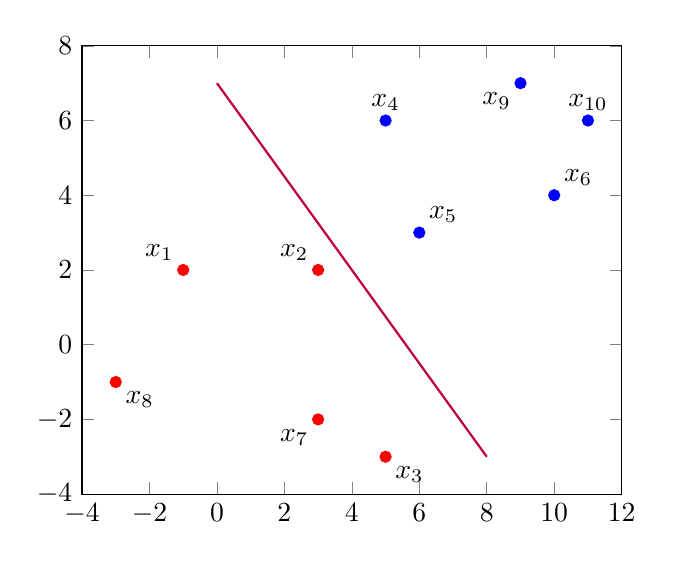
\begin{tikzpicture}
        \begin{axis}[
            axis lines = box,
            xmin=-4, xmax=12,
            ymin=-4, ymax=8,
        ]
    
        % Синие точки
        \addplot[only marks, mark=*, color=blue] coordinates {(5, 6) (6, 3) (10, 4) (9, 7) (11, 6)};
        \node[black] at (axis cs:5, 6) [above] {$x_4$};
        \node[black] at (axis cs:6, 3) [above right] {$x_5$};
        \node[black] at (axis cs:10, 4) [above right] {$x_6$};
        \node[black] at (axis cs:9, 7) [below left] {$x_9$};
        \node[black] at (axis cs:11, 6) [above] {$x_{10}$};
    
        % Красные точки
        \addplot[only marks, mark=*, color=red] coordinates {(-1, 2) (3, 2) (5, -3) (3, -2) (-3, -1)};
        \node[black] at (axis cs:-1, 2) [above left] {$x_1$};
        \node[black] at (axis cs:3, 2) [above left] {$x_2$};
        \node[black] at (axis cs:5, -3) [below right] {$x_3$};
        \node[black] at (axis cs:3, -2) [below left] {$x_7$};
        \node[black] at (axis cs:-3, -1) [below right] {$x_8$};
    
        % Фиолетовый отрезок
        \addplot[color=purple, thick] coordinates {(8, -3) (0, 7)};
        
        \end{axis}
    \end{tikzpicture}
    \caption{линейный классификатор без ошибок}
    \label{fig:pic1}
  \end{figure}

  \begin{figure}[hbt!]
    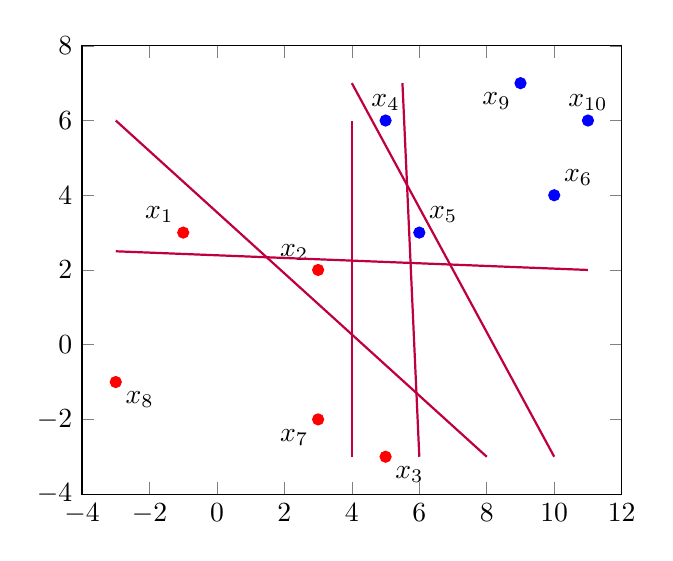
\begin{tikzpicture}
        \begin{axis}[
            axis lines = box,
            xmin=-4, xmax=12,
            ymin=-4, ymax=8,
        ]
    
        % Синие точки
        \addplot[only marks, mark=*, color=blue] coordinates {(5, 6) (6, 3) (10, 4) (9, 7) (11, 6)};
        \node[black] at (axis cs:5, 6) [above] {$x_4$};
        \node[black] at (axis cs:6, 3) [above right] {$x_5$};
        \node[black] at (axis cs:10, 4) [above right] {$x_6$};
        \node[black] at (axis cs:9, 7) [below left] {$x_9$};
        \node[black] at (axis cs:11, 6) [above] {$x_{10}$};
    
        % Красные точки
        \addplot[only marks, mark=*, color=red] coordinates {(-1, 3) (3, 2) (5, -3) (3, -2) (-3, -1)};
        \node[black] at (axis cs:-1, 3) [above left] {$x_1$};
        \node[black] at (axis cs:3, 2) [above left] {$x_2$};
        \node[black] at (axis cs:5, -3) [below right] {$x_3$};
        \node[black] at (axis cs:3, -2) [below left] {$x_7$};
        \node[black] at (axis cs:-3, -1) [below right] {$x_8$};
    
        % Фиолетовый отрезок
        \addplot[color=purple, thick] coordinates {(4, -3) (4, 6)};
        \addplot[color=purple, thick] coordinates {(4, 7) (10, -3)};
        \addplot[color=purple, thick] coordinates {(6, -3) (5.5, 7)};
        \addplot[color=purple, thick] coordinates {(-3, 2.5) (11, 2)};
        \addplot[color=purple, thick] coordinates {(8, -3) (-3, 6)};
        
        \end{axis}
    \end{tikzpicture}
    \caption{линейный классификатор с 1 ошибкой}
    \label{fig:pic2}
  \end{figure}

\begin{table}[hbt!]
    \begin{tabular}{c|c|ccccc|c}
		$x_1$ & 0 & 1 & 0 & 0 & 0 & 0 & \dots \\
    $x_2$ & 0 & 0 & 1 & 0 & 0 & 0 & \dots \\
		$x_3$ & 0 & 0 & 0 & 1 & 0 & 0 & \dots \\
    $x_4$ & 0 & 0 & 0 & 0 & 1 & 0 & \dots \\
    $x_5$ & 0 & 0 & 0 & 0 & 0 & 1 & \dots \\
    $x_6$ & 0 & 0 & 0 & 0 & 0 & 0 & \dots \\
    $x_7$ & 0 & 0 & 0 & 0 & 0 & 0 & \dots \\
    $x_8$ & 0 & 0 & 0 & 0 & 0 & 0 & \dots \\
    $x_9$ & 0 & 0 & 0 & 0 & 0 & 0 & \dots \\
    $x_{10}$ & 0 & 0 & 0 & 0 & 0 & 0 & \dots \\
    \end{tabular}
    \caption{матрица ошибок для примера 1}
\end{table}

Наша задача будет оценивать вероятность переобучения. Для начала дадим несколько определений.
Вероятностное пространтво $-$ это равновероятное разбиение выборки на 2 части (train $X^l$ и test $X^k$). Интерпретация этому это гипотеза, что наша выборка IID (independent and identically distributed). Т. е. как бы мы эту выборку не упорядочивали, все ее упорядочивания равновероятны (как бы мы ее не разбивали на две части, все разбиения равновероятны). Это есть гипотеза простой выборки.

\textit{Замечание.} С другой стороны на это можно смотреть, как на Complete Cross Validation (полный скользящий контроль). Всеми способами разбиваем выборку на train и test. Потом по всем этим способам вероятность любого события, зависящая от этого разбиения, усредняем по всем разбиениям. В этой вероятностной интерпретации очень удобно, что математическое ожидание есть просто усреднение по всем разбиениям выборки
\begin{equation*}
    P \equiv E \equiv \frac{1}{C_L^l} \sum_{X^l \subset X^L}.
\end{equation*}

Переобученность $-$ это разность частот ошибок на $X^k$ и на $X^l$ (обучились на $X^l$, частоту ошибок посчитали на $X^k$, частота ошибок нормирована от 0 до 1):
\begin{equation*}
    \delta (\mu, X^l, X^k)=\nu (\mu(X^l), X^k ) - \nu(\mu(X^l), X^l ).
\end{equation*}

Переобучение $-$ это событие $\delta (\mu, X^l, X^k) \geq \varepsilon$ для фиксированного $\varepsilon$.

Основная наша задача $-$ оценить \textit{вероятность} переобучения (вероятность в смысле доли разбиения выборки, на которых $\delta$ оказалась $\geq \varepsilon$ при заданном $\varepsilon$):
\begin{equation*}
    R_{\varepsilon}(\mu, X^L) = P [\delta(\mu, X^l, X^k) \geq \varepsilon].
\end{equation*}

Теперь наша задача $-$ научиться сверху оценивать эту величину. Рассмотрим простейший, но важный частный случай.

Пусть у нас нет никакого выбора алгоритма, научимся оценивать вероятность переобучения хотя бы для одного отдельно взятого алгоритма, т. е. для одного вектор-столбца матрицы ошибок.
Пусть $A = {a}$ $-$ одноэлементарное множество, $m=n(a, X^L)$. Тогда вероятность переобучения есть вероятность большого отклонения частот ошибок в двух подвыборках:

\begin{equation*}
    R_{\varepsilon}(a, X^L) = P [\nu(a, X^k) - \nu(a, X^l) \geq \varepsilon].
\end{equation*}

\textbf{Теорема} Для любой выборки $X^l$, любого $\varepsilon \in [0, 1]$ вероятность большого отклонения частот ошибок в двух подвыборках для фиксированного вектора ошибок:
$$R_{\varepsilon}(a, X^L)=\mathcal{H}_L^{l, m}(\frac{l}{L}(m-\varepsilon k)),$$
где $\mathcal{H}_L^{l, m}(x)=\sum_{s=0}^{\lfloor x \rfloor}\frac{C_m^s C_{L-m}^{l-s}}{C_L^l}$ $-$ функция гипергеометрического распределения (ее левый хвост).

\textbf{Доказательство.}
$\square$ Обозначим число ошибок на обучении как $s=n(a, X^l)$. Аналогия со 2 задачей из упражнения,  где $m$ $-$ количество объектов с ошибками, $l$ $-$ обучающая выборка (гипергеометрическое распределение):
\begin{equation*}
    P[n(a, X^l)=s]=C_m^s C_{L-m}^{l-s}/C_L^l.
\end{equation*}
Распишем $R_{\varepsilon}$, подставив в него $\nu(a, X^k)=\frac{m-s}{k}$, $\nu(a, X^l)=\frac{s}{l}$ (частота ошибок на обучении $\frac{s}{l}$, а на контроле $\frac{m-s}{k}$) и учитывая тот факт, что $\frac{m-s}{k}-\frac{s}{l}$ есть переобученность:
\begin{multline*}
    R_{\varepsilon}(a, X^L)=P[\nu(a, X^k)-\nu(a, X^l) \geq \varepsilon] = \\
    = \sum_{s=0}^l [\underbrace{\frac{m-s}{k}-\frac{s}{l} \geq \varepsilon}_{s \leq \frac{l}{L}(m-\varepsilon k)}]\underbrace{P[n(a, X^l)=s]}_{C_m^s C_{L-m}^{l-s}/C_L^l}=\mathcal{H}_L^{l, m}(\frac{l}{L}(m-\varepsilon k)).
\end{multline*}

При это мы получили ограничение на $s$, которое является следствием того, что переобученность $\leq \varepsilon$. Наша оценка $-$ левый хвост гипергеометрического распределения.
$\blacksquare$

Посмотрим как это выглядит на картинке. На оси $x$ отложено $m$ $-$ общее число ошибок на полной выборке, по оси $y$ откладывается число ошибок на обучающей выборке. На графике \ref{fig:pic3} видна узкая полоска $-$ \textit{явление концентрации вероятностной меры}. Это очень важное явление и в теории вероятности, и в машинном обучении, и в Computational learning theory. Это основной теоретический момент, из которого могут быть получены различные оценки (красная полоска). При том чем больше будет длина выборки, тем уже будет относительная ширина этой полоски.

Предсказание числа $m=n(a, X^L)$ по числу $s=n(a, X^l)$ возможно благодаря узости гипергеометрического пика, причем при $l,k \rightarrow \infty$ он сужается, и $\nu(a, X^l) \rightarrow \nu(a, X^k)$ (явление концентрации вероятности, закон больших чисел).

Гипергеометрическое распределение нам говорит, что если мы знаем $m$ (общее число ошибок на полной выборке), то мы можем предсказать диапазон изменений для $s$, т. е. сколько у нас ошибок попадет в обучение. Значит будем знать $m-s$, сколько ошибок попадет в контроль. Но в реальной ситуации нам приходиться обращать это гипергеометрическое распределение, т. к. мы знаем сколько ошибок у нас попало в обучение. Мы знаем что у нас по $y$ и можем провести горизонтальную линию и сказать, в каком у нас диапазоне могло бы быть $m$, т. е. в каком диапазоне могло бы лежать общее число ошибок на объединенной выборке. А $m-s$ это число ошибок на контроле.

\usetikzlibrary{intersections}
\usepgfplotslibrary{fillbetween}

\begin{figure}[hbt!]
    \centering
    \begin{subfigure}[t]{0.45\textwidth}
        \centering
        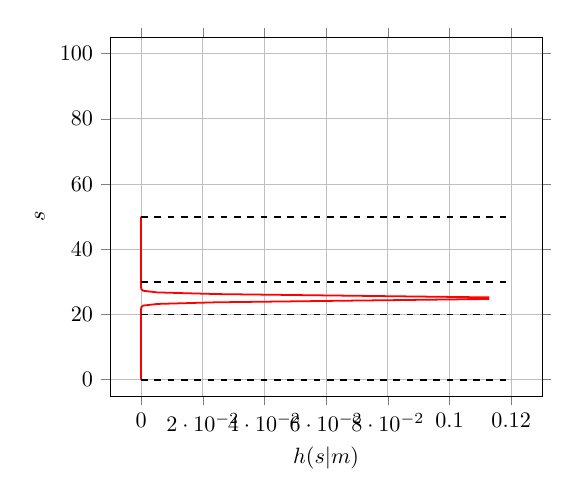
\begin{tikzpicture}[scale=0.8]
            \begin{axis}[
                grid=both,
                xlabel={$h(s|m)$},
                ylabel={$s$},
                ymin=-5, ymax=105,
                xmin=-0.01, xmax=0.13,
                tick align=outside
            ]
                \addplot[red, thick, domain=0:50, samples=100] (0.12*exp(-(x-25)*(x-25)),x);
                \addplot[color=black, thick, dashed] coordinates {(0, 0) (0.12, 0)};
                \addplot[color=black, thick, dashed] coordinates {(0, 20) (0.12, 20)};
                \addplot[color=black, thick, dashed] coordinates {(0, 30) (0.12, 30)};
                \addplot[color=black, thick, dashed] coordinates {(0, 50) (0.12, 50)};
            \end{axis}
        \end{tikzpicture}
        \caption{$h(s|m)$ при $m=50$}
        \label{fig:pic3}
    \end{subfigure}\hfill
    \begin{subfigure}[t]{0.45\textwidth}
        \centering
        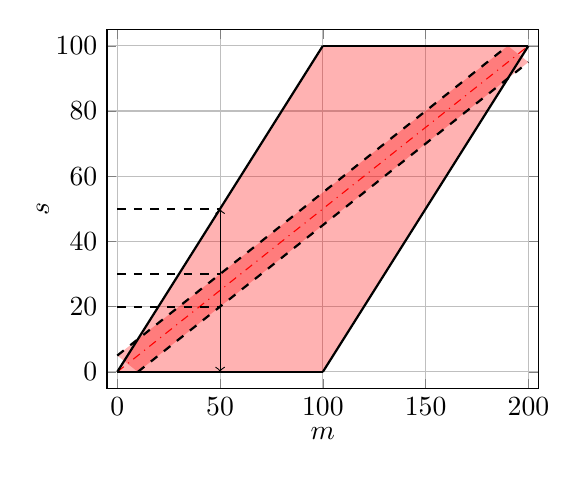
\begin{tikzpicture}[scale=0.8]
            \begin{axis}[
                grid=both,
                xlabel={$m$},
                ylabel={$s$},
                xmin=-5, xmax=205,
                ymin=-5, ymax=105,
            ]
                % Main diagonal
                \addplot[red, domain=0:200, samples=100, dashdotted] {x/2};
                % Shaded region
                \addplot[name path=A, domain=10:200, samples=100, thick, dashed] {x/2 - 5};
                \addplot[name path=B, domain=0:190, samples=100, thick, dashed] {x/2 + 5};
    
                \addplot[name path=seg1, color=black, thick] coordinates {(0, 0) (100, 100)};
                \addplot[name path=seg2, color=black, thick] coordinates {(100, 100) (200, 100)};
                \addplot[name path=seg3, color=black, thick] coordinates {(200, 100) (100, 0)};
                \addplot[name path=seg4, color=black, thick] coordinates {(100, 0) (0, 0)};
                \addplot[red, opacity=0.3] fill between[of=seg1 and seg4];
                \addplot[red, opacity=0.3] fill between[of=seg2 and seg3];
    
                \addplot[red, opacity=0.3] fill between[of=A and B];
                \addplot[color=black, thick, dashed] coordinates {(0, 50) (50, 50)};
                \addplot[color=black, thick, dashed] coordinates {(0, 30) (50, 30)};
                \addplot[color=black, thick, dashed] coordinates {(0, 20) (50, 20)};
                \addplot[color=black, thick, dashed] coordinates {(0, 0) (50, 0)};
                \addplot[color=black, <->] coordinates {(50, 0) (50, 50)};
            \end{axis}
        \end{tikzpicture}
        \caption{$h(s|m)$ при $L=200, k=100$}
        \label{fig:pic4}
    \end{subfigure}
    \caption{Гипергеометрическое распределение $h(s|m)$}
\end{figure}

\textbf{Задача 1.} Сколько линейных классификаторов с двумя ошибками из примера 1?

\textbf{Решение.}

Для решения задачи необходимо посмотреть сколько существует различных способов разделить объекты на рисунке \ref{fig:pic1}, чтобы объектов одного класса было на 2 больше, чем другого. Приведем ответ в виде таблицы:

\begin{table}[hbt!]
    \begin{tabular}{c|cccccccc}
		$x_1$ & 1 & 0 & 0 & 0 & 0 & 1 & 1 & 0 \\
    $x_2$ & 1 & 1 & 0 & 0 & 0 & 0 & 0 & 0 \\
		$x_3$ & 0 & 1 & 1 & 0 & 0 & 0 & 0 & 1 \\
    $x_4$ & 0 & 0 & 1 & 1 & 0 & 0 & 0 & 0 \\
    $x_5$ & 0 & 0 & 0 & 1 & 1 & 1 & 0 & 0 \\
    $x_6$ & 0 & 0 & 0 & 0 & 1 & 0 & 1 & 0 \\
    $x_7$ & 0 & 0 & 0 & 0 & 0 & 0 & 0 & 1 \\
    $x_8$ & 0 & 0 & 0 & 0 & 0 & 0 & 0 & 0 \\
    $x_9$ & 0 & 0 & 0 & 0 & 0 & 0 & 0 & 0 \\
 $x_{10}$ & 0 & 0 & 0 & 0 & 0 & 0 & 0 & 0 \\
    \end{tabular}
    \caption{все возможные разбиения с 2 ошибками}
\end{table}

\textbf{Задача 2.} В урне $L$ шаров, $m$ из них черные, остальные белые; извлекаем $l$ шаров наугад. Какова вероятность, что ровно $s$ из них черные?

\textbf{Решение.}

Обозначим:
$N = L$ $-$ общее количество шаров в урне,
$m$ $-$ количество черных шаров,
$N - m$ $-$ количество белых шаров,
$l$ $-$ общее количество извлеченных шаров,
$s$ $-$ количество черных шаров среди извлеченных.

Чтобы найти вероятность, нам нужно рассмотреть, сколько способов существует для выбора $s$ черных шаров и $l - s$ белых шаров из общего количества.

Выбрать $s$ черных шаров из $m$ черных можно $C_m^s$ способами.

А выбрать $l - s$ белых шаров из $N - m$ белых $-$ $ C_{N - m}^{l - s}$ способами.

Общее количество способов выбрать $l$ шаров из $N$ есть $C_N^l$.

Таким образом, вероятность того, что из $l$ извлеченных шаров ровно $s$ будут черными, будет равна отношению числа благоприятных исходов к общему числу исходов:

$$
P(X = s) = \frac{C_{m}^{s} \cdot C_{N - m}^{l - s}}{C_{N}^{l}}
$$

\textbf{Задача 3.} Как посчитать количество рыб в пруду?

\textbf{Решение.} Выловим некоторое случайное подмножество рыб, пометим их, а потом выпустим обратно в пруд. Через некоторое время рыбы в пруду перемешаются (важно, чтобы они успели перемешаться), опять вылавливаем некоторое количество рыб и смотрим, какая доля среди них $-$ меченная. По этим данным, очевидно, можно найти общее количество рыб в пруду.


\section{Статистические критерии в машинном обучении}
\subsection{Теория}

Статистические инструменты используются для отбора, извлечения и преобразования наиболее релевантных признаков. Например, коэффициент корреляции Пирсона, ранговый коэффициент Спирмена, коэффициент корреляции ANOVA, ранговый коэффициент Кендалла и критерий  Хи-квадрат \\

В данном обзоре рассмотрим приложения математической статистики в машинном обучении – точнее, в отборе признаков для обучения модели.  \\

Мотивация: Преимущества хорошо подобранных признаков в датасете очевидны: это улучшает точность в обучении с учителем и без, уменьшает время и память, необходимые для корректной работы, помогает ослабить проклятие размерности (экспоненциальный рост необходимых данных). \\

Одним из основных методов, используемых для отбора признаков, является анализ корреляции. Корреляция позволяет определить, насколько сильно связаны между собой различные признаки и целевая переменная. Признаки с высокой корреляцией с целевой переменной могут быть отобраны для дальнейшего анализа, в то время как признаки, которые не имеют значительной связи, могут быть исключены. Это помогает избежать проблем многоколлинеарности, когда несколько признаков предоставляют одинаковую информацию.\\

Другим важным инструментом является тестирование гипотез. С помощью статистических тестов, таких как t-тест или ANOVA, можно оценить значимость отдельных признаков в контексте целевой переменной. Например, если мы имеем дело с задачей классификации, мы можем использовать тесты для определения того, какие признаки значительно различаются между классами. Это позволяет сосредоточиться на наиболее информативных признаках и исключить те, которые не вносят существенного вклада в модель.\\

Методы селекции на основе значимости также широко применяются в практике. Алгоритмы, такие как LASSO (Least Absolute Shrinkage and Selection Operator), используют регуляризацию для уменьшения коэффициентов менее значимых признаков до нуля, что автоматически исключает их из модели. Это не только упрощает модель, но и помогает избежать переобучения — проблемы, когда модель слишком точно подстраивается под обучающие данные и теряет способность обобщать на новых данных.\\

Методы оценки производительности модели также зависят от правильного отбора признаков. Кросс-валидация позволяет оценить, как изменения в наборе признаков влияют на общую производительность модели. Сравнение различных моделей с разными наборами признаков помогает выбрать оптимальный вариант, который обеспечивает наилучшие результаты.\\

Кроме того, современные подходы к машинному обучению, такие как ансамблевые методы (например, Random Forest), также используют статистические методы для оценки важности признаков. В таких методах важность каждого признака может быть оценена по тому, как сильно он влияет на уменьшение ошибки предсказания модели. \\

\subsection{Задачи}

1. Анализ корреляции\\
У вас есть набор данных с 5 признаками (X1, X2, X3, X4, X5) и целевой переменной Y. Вы хотите выяснить, какие признаки имеют наибольшую корреляцию с Y.

\textit{Решение:\\
1. Рассчитайте коэффициенты корреляции Пирсона для каждого признака относительно Y.\\
2. Сравните полученные значения и выберите признаки с наибольшими абсолютными значениями коэффициента корреляции.}
   
2. Тестирование гипотез\\
Вы хотите проверить, есть ли статистически значимая разница между двумя группами данных (группа A и группа B) по признаку X. У вас есть данные о значениях X для обеих групп.

\textit{Решение:\\
1. Проведите t-тест для независимых выборок.\\
2. Оцените p-значение для определения значимости.}

3. Регуляризация LASSO \\
У вас есть набор данных с несколькими признаками и целевой переменной. Вы хотите использовать метод LASSO для отбора наиболее значимых признаков.

\textit{Решение:\\
1. Импортируйте библиотеку Lasso из sklearn.\\
2. Подготовьте данные и обучите модель LASSO.\\
3. Оцените важность признаков на основе полученных коэффициентов.\\}


\section{Кросс-валидация}

\subsection{Теория}

Кросс-валидация — это процедура для оценки качества работы модели, которая позволяет более точно оценивать, как модель будет работать на новых, невидимых данных. Основная идея заключается в разбиении данных на несколько частей и обучении модели на разных комбинациях этих частей. При этом  проверять качество модели необходимо на оставшихся данных.

\subsubsection{Hold-out}

В этом методе данные просто разделяются на train и test. После этого происходит обучение на train и проверка качества на test. При этом важно перемешивать данные, потому что в противном случае могут появиться неожиданные <<спецэффекты>>. Например, в изначальных данные может быть, что первые 80\% --- это изображения с кошками, а остальные 20\% --- с собаками. Если при этом цель --- научить модель различать кошек и собак, то очень важные всё перемешать, чтобы не оказалось, что в train попали только кошки.

\begin{figure}[h]
	\centering
	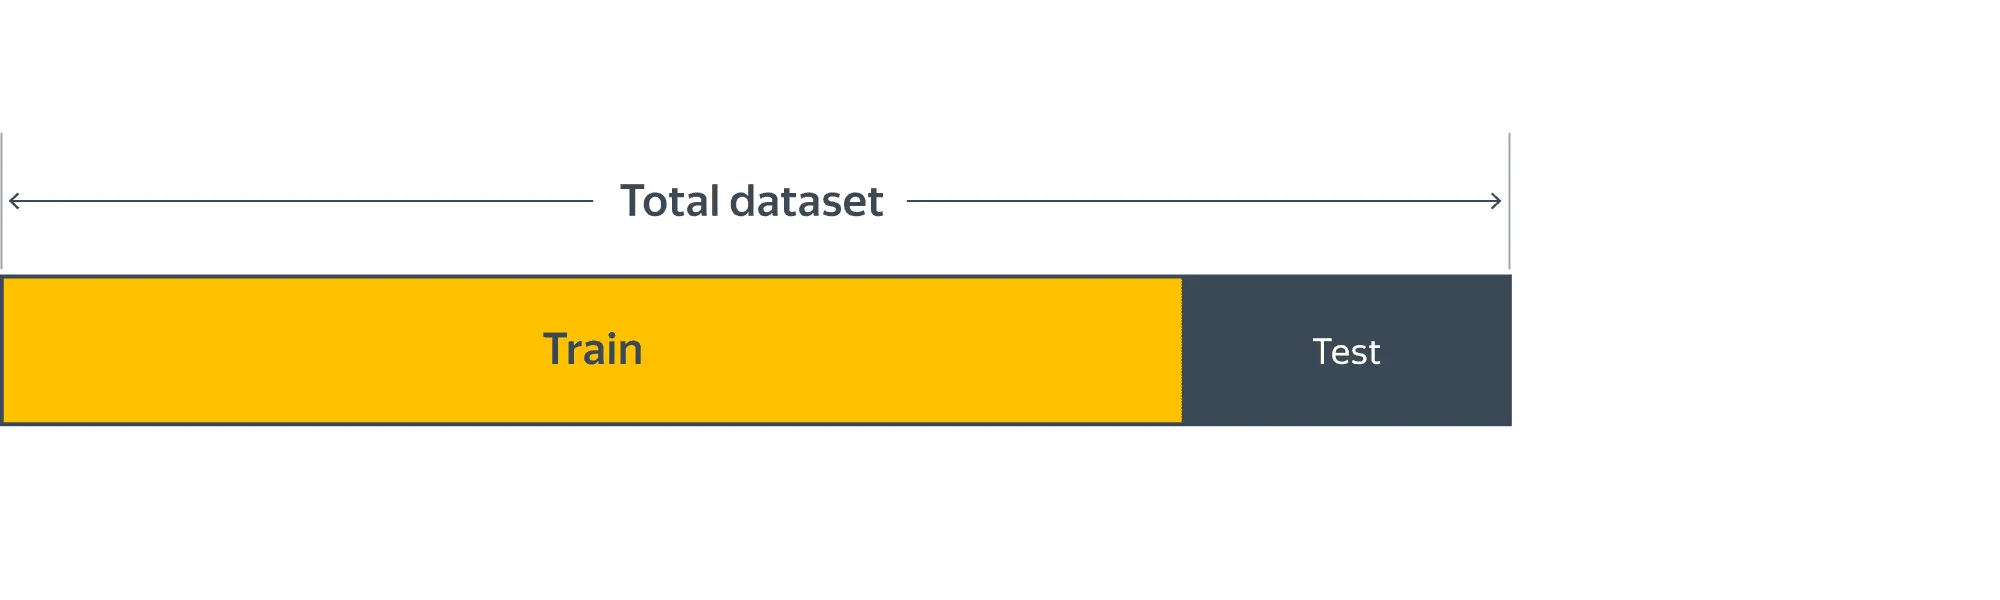
\includegraphics[width=\textwidth/2]{hold_out.png}
	\caption{Hold-out}
	\label{img:hold-out}
\end{figure}

\subsubsection{k-Fold}

Это самый распространенный метод кросс-валидации, в нём данные разбиваются на k подмножеств. Модель обучается k раз, каждый раз используя одно подмножество в качестве тестовой выборки, а остальные k-1 как тренировочные. В конце ошибкой модели считается либо средняя полученная ошибка по всем выборам тестового множества, либо вычисляется на отдельно отложенном валидационном множестве. Это позволяет использовать все доступные данные для обучения и тестирования, что особенно полезно в случаях, когда данные ограничены.

\begin{figure}[h]
	\centering
	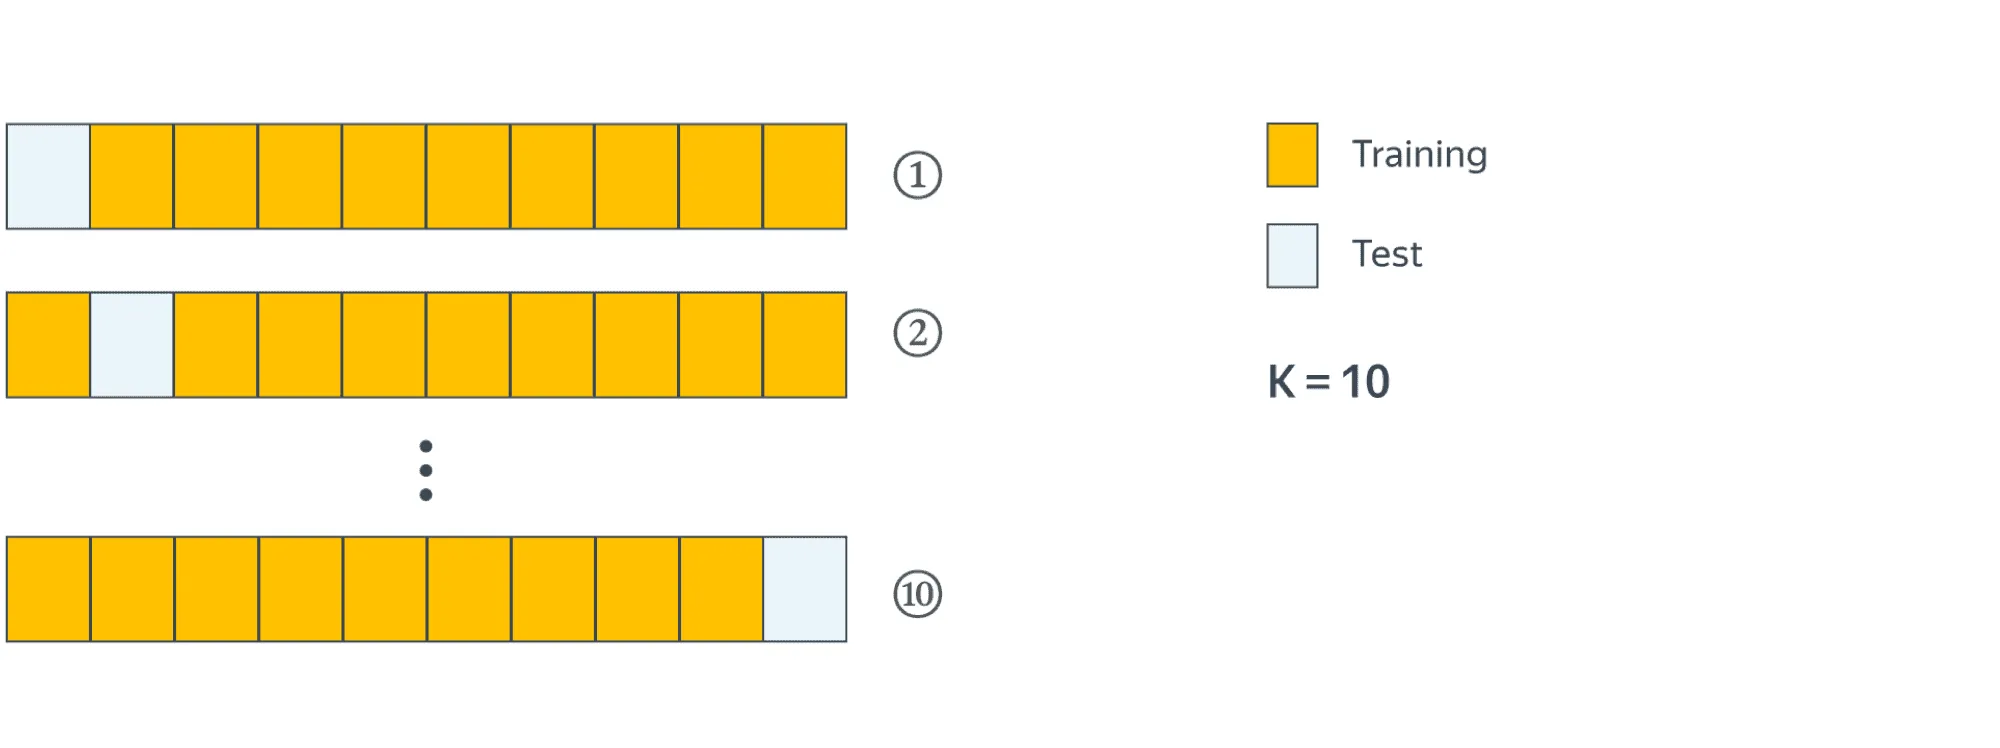
\includegraphics[width=\textwidth/2]{k-fold.png}
	\caption{k-Fold}
	\label{img:k-fold}
\end{figure}

Можно сделать вывод, что кросс-валидация помогает избежать переобучения и оптимизировать гиперпараметры моделей засчёт того, что модель много раз обучается и тестируется на разных подмножествах одних и тех же данных.

\subsection{Задачи (\href{https://education.yandex.ru/handbook/ml/article/kross-validaciya}{источник})}

\subsubsection{Задача 1}
Пример из практики Yandex.Research — как вы думаете, что не так с графиком обучения данной модели?

\begin{figure}[h]
	\centering
	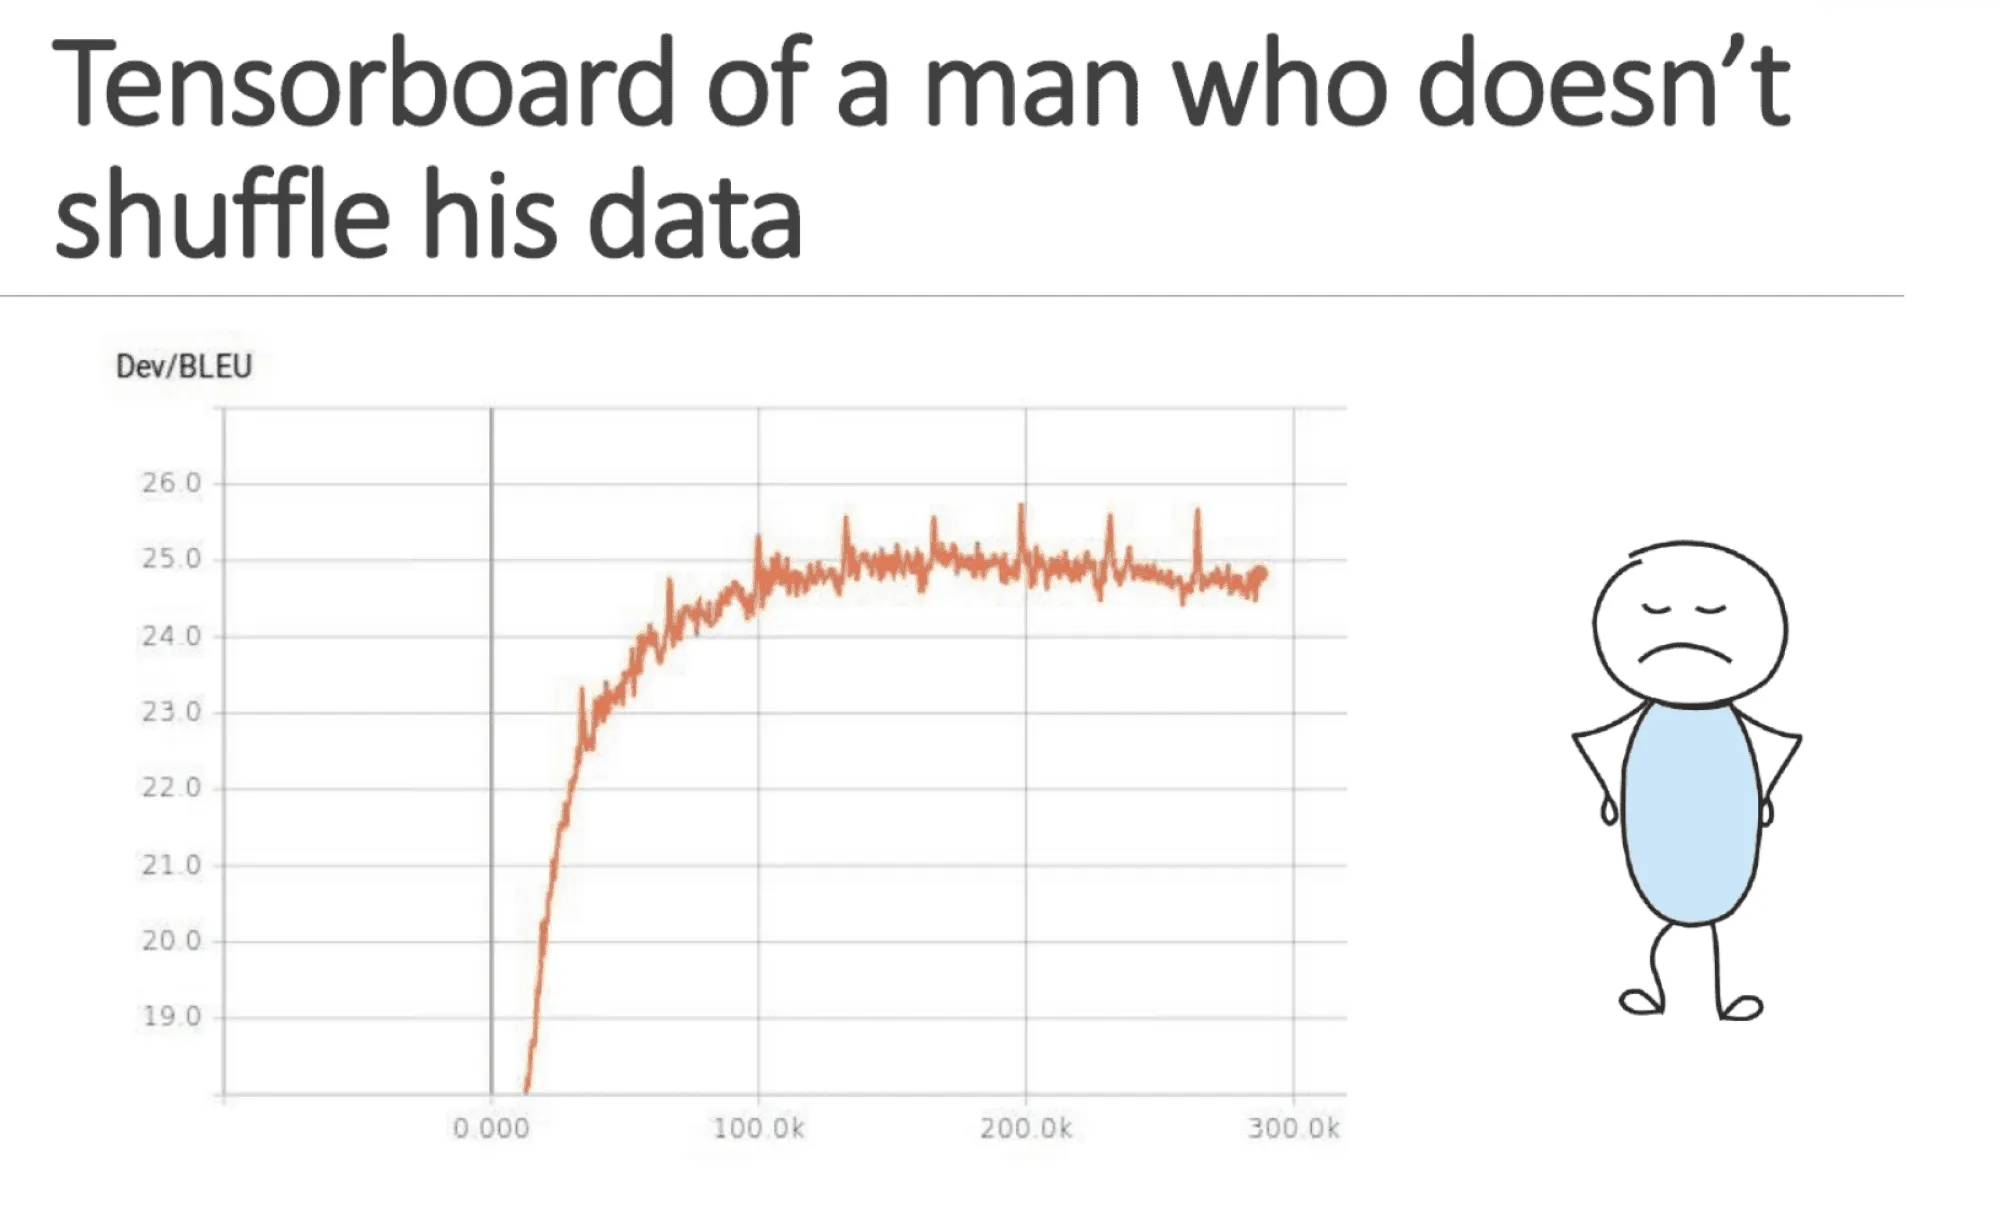
\includegraphics[width=\textwidth/2]{problem-1.png}
	\caption{Задача 1}
	\label{img:problem-1}
\end{figure}

\textit{Решение}
На графике видна периодичность по числу итераций! По большим пикам можно вычислить места, где проход по данным начался заново. Кроме того, график в конце ползёт вниз, что означает, что модель уже начала переобучаться, выучив последовательность данных на трейне и используя эту информацию больше, чем сами данные.

Если данные перемешать, то график обучения станет таким:

\begin{figure}[h]
	\centering
	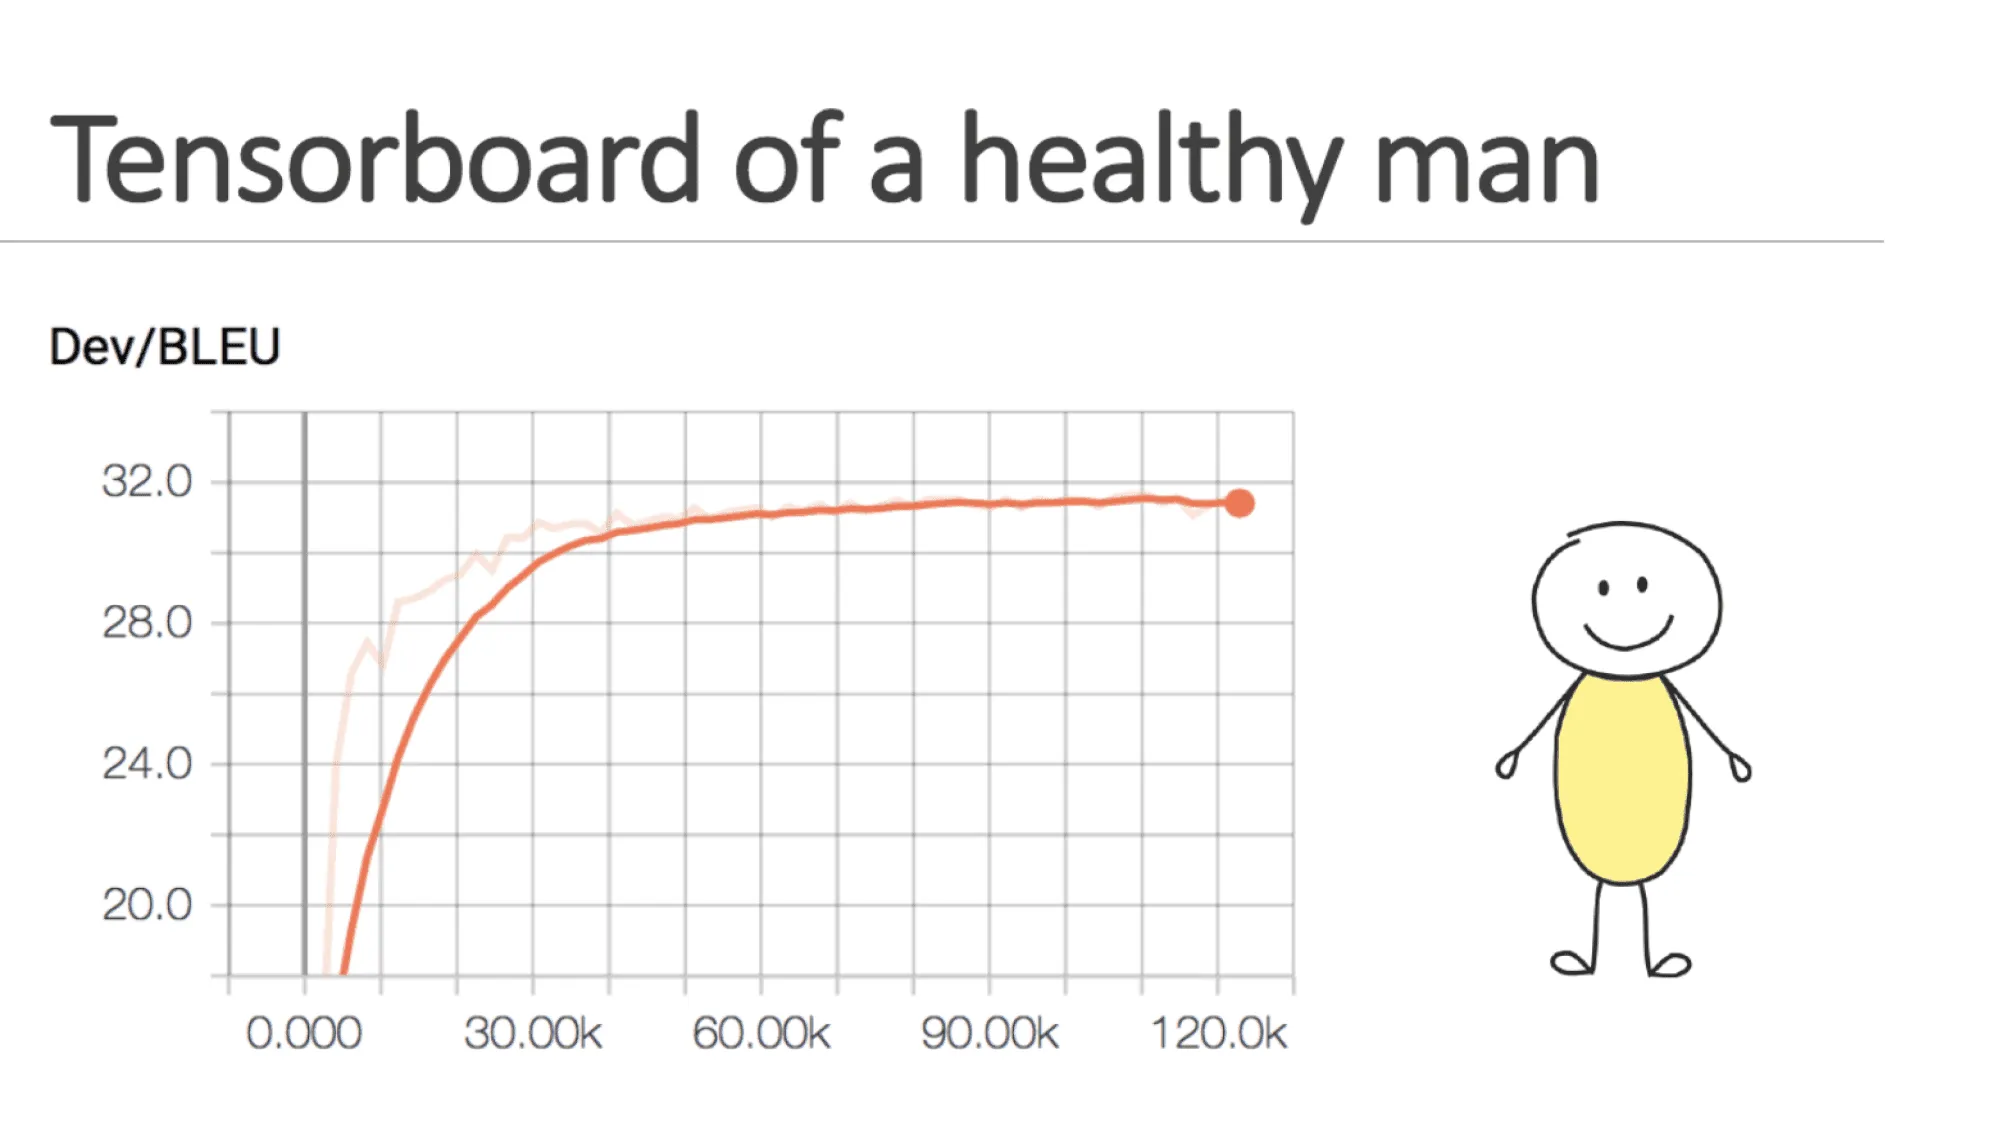
\includegraphics[width=\textwidth/2]{sol-1.png}
	\caption{Решение задачи 1}
	\label{img:sol-1}
\end{figure}

\subsubsection{Задача 2}

Пусть нужно обучить модель, которая должна предсказывать погоду. Есть исторические данные за последние 10 лет. Можно ли как обычно разделять данные на train и test, произвольно перемешивая их? Если нет, то как нужно разделять данные?

\textit{Решение}
Нет, так делать нельзя, потому что в таком случае у модели при обучении будет доступ к данным из <<будущего>>, которые он как раз и должна предсказывать, а это некорректно. Правильно будет разделить данные по времени: самые старые --- train, самые новые -- test.

\subsubsection{Задача 3}

А как сделать кросс-валидацию в условиях задачи 2?

\textit{Решение}

Нужно сделать несколько пар (train, test), но так, чтобы модель никогда не получала лишних данных из будущего. С учётом особенностей фолды в кросс-валидации для временных рядов располагаются вдоль временной оси так, как показано на следующей картинке:

\begin{figure}[h]
	\centering
	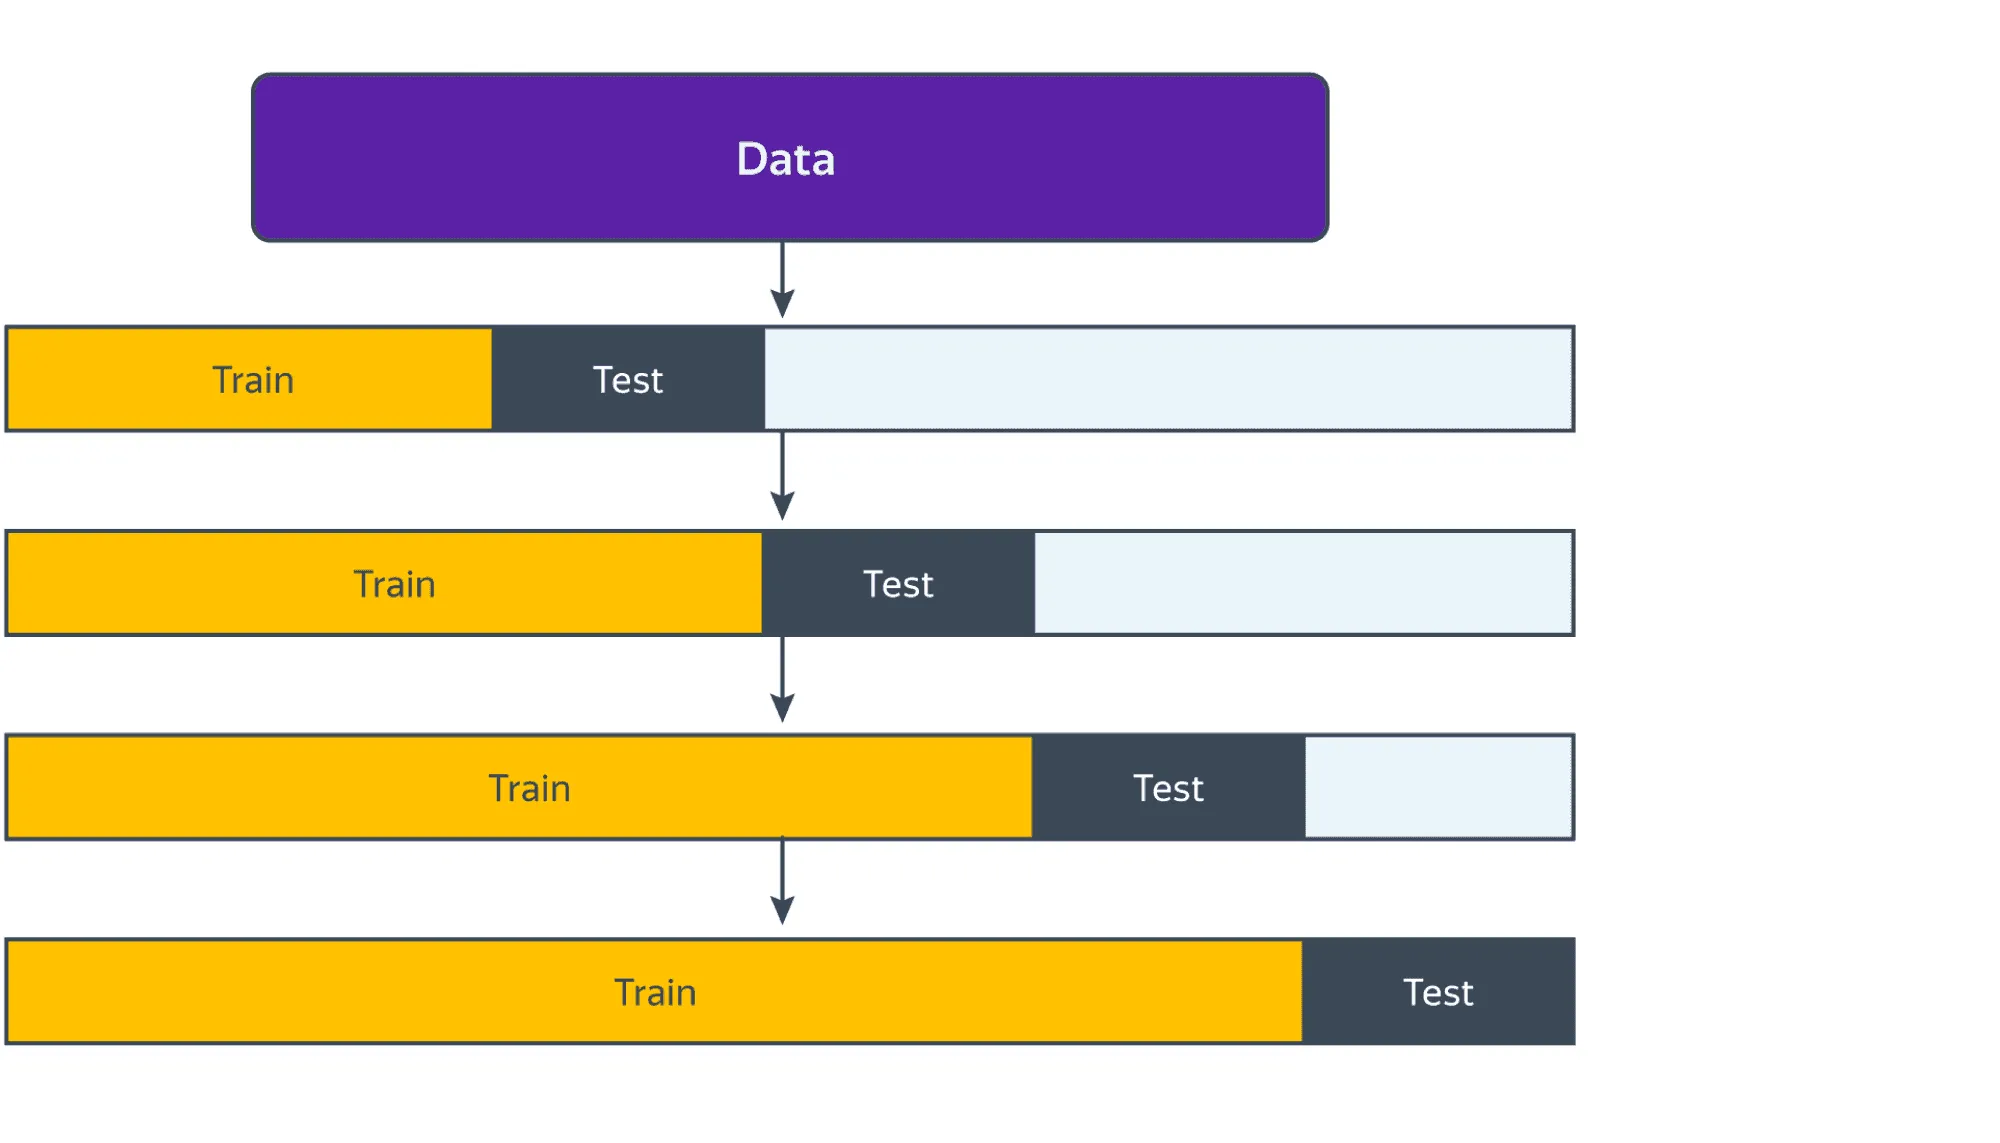
\includegraphics[width=\textwidth/2]{sol-3.png}
	\caption{Решение задачи 3}
	\label{img:sol-3}
\end{figure}





\section{Квазиньютоновские методы и методы BFGS и L-BFGS}
\section*{Введение}
Метод Ньютона для размерности $d > 1000$ уже не является эффективным, поскольку требует вычисления и хранения гессиана, а также решения системы линейных уравнений с его участием (что может быть в общем случае очень дорого). Однако существуют квазиньютоновские методы, такие как BFGS и L-BFGS. \\
BFGS — один из наиболее широко применяемых квазиньютоновских методов. В нем гессиан, вместо вычисления напрямую оценивается приближенно. L-BFGS - модификация данного метода с ограниченным использованием памяти которая предназначена для решения нелинейных задач с большим количеством неизвестных.



\section*{Метод секущей и общая схема квазиньютоновских методов}
Перед тем как перейти к  BFGS и L-BFGS рассмотрим метод секущей.
Пусть мы хотим найти такую точку $x^*$, что $g(x^*)=0$. В одномерном случае мы можем подменить вычисление $g'(x_n)$ вычислением её приближения $(g(x_n) - g(x_{n-1}))/(x_n - x_{n-1})$. Откуда получаем формулу пересчета:

\[x_{n+1} = x_n - \frac{x_n - x_{n-1}}{g(x_n) - g(x_{n-1})}g(x_n)\]


Графически, этот метод выглядит следующим образом:

\begin{center}
  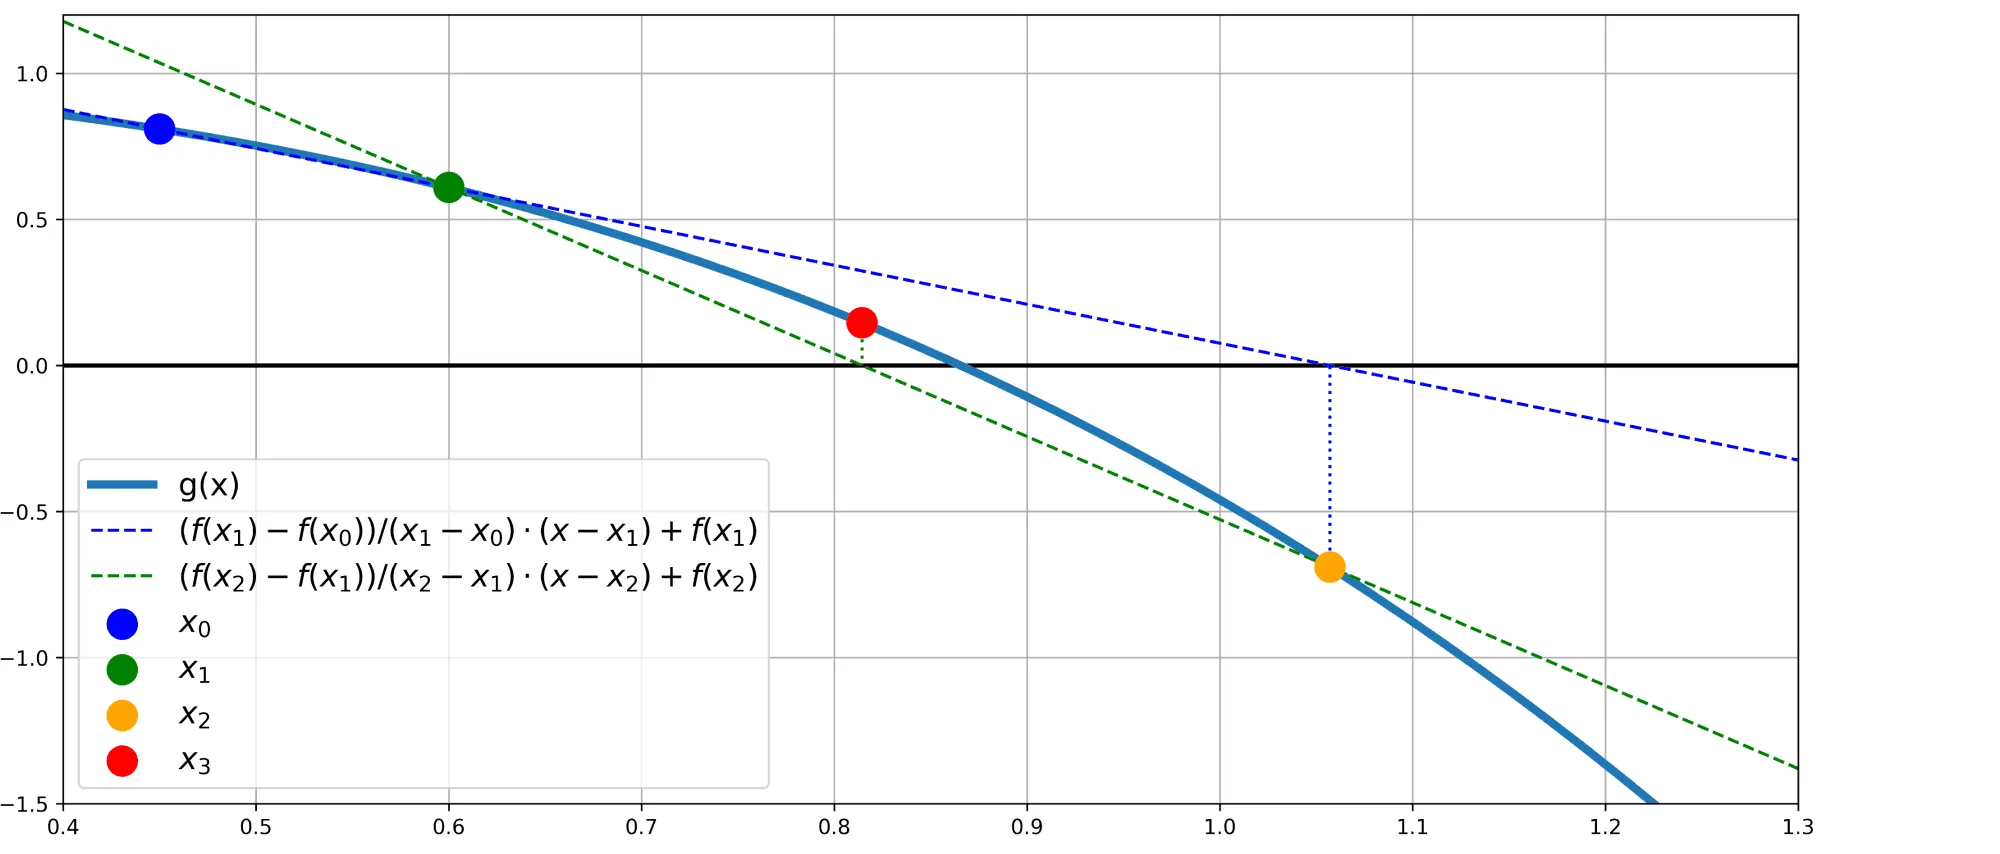
\includegraphics[width=0.7\textwidth]{secant_method.png}
\end{center}
  
Скорость сходимости этого метода несколько ниже, чем у метода Ньютона (линейная, а не квадратичная), но зато мы теперь не должны вычислять производную. По сути проводим через два предыдущих приближения секущую, а затем выбираем ноль этой секущей в качестве следующей точки.

В многомерном случае мы можем выписать соответствующее уравнение
\[
y = B_k \left( x - x^k \right) + g(x^k),
\]
где \( B_k \) — матрица размера \( d \times d \), которая должна удовлетворять так называемому уравнению секущей (secant equation):
\[
B_k \left( x^k - x^{k-1} \right) = g(x^k) - g(x^{k-1}).
\]

Теперь, чтобы выбрать следующую точку, нужно найти ноль секущей, то есть
\[
B_k \left( x^{k+1} - x^k \right) + g(x^k) = 0 
\quad \Longleftrightarrow \quad 
x^{k+1} = x^k - B_k^{-1} g(x^k).
\]

А теперь рассмотрим \( g(x) = \nabla f(x) \) и добавим в итеративную схему выше размер шага. Тогда мы получаем общую итеративную схему квазиньютоновских методов:
\[
x^{k+1} = x^k - \alpha_k B_k^{-1} \nabla f(x^k).
\]

При этом необходимо выбирать такие \( B_k \), чтобы они
\begin{enumerate}
    \item были симметричными и положительно определёнными и
    \item удовлетворяли уравнению секущей
    \[
    B_k \left( x^k - x^{k-1} \right) = \nabla f(x^k) - \nabla f(x^{k-1}).
    \]
\end{enumerate}

Теперь рассмотрим широко известный метод \textbf{BFGS} (Broyden, Fletcher, Goldfarb, Shanno).



\section*{BFGS}

Сначала заметим, что в самом алгоритме в первую очередь используется обратная матрица к $B_k$, которую мы обозначим $H_k = B_k^{-1}$. Тогда выбирать $B_k$ — это тоже самое, что выбирать $H_k$. Введем еще два стандартных обозначения, чтобы можно было проще записывать все последующие формулы: 
\[
s_k = x_{k+1} - x_k = \alpha_k d_k, \quad y_k = \nabla f(x^{k+1}) - \nabla f(x^k).
\]
В их терминах уравнение секущей для $H_k$ выглядит максимально просто: 
\[
H_k y_{k-1} = s_{k-1}.
\]

Теперь введем некоторое искусственное требование, которое гарантирует единственность $H_{k+1}$ — выберем ближайшую подходящую матрицу к $H_k$, удовлетворяющую описанным выше условиям:
\[
H_{k+1} = \arg\min_H \left\{ \frac{1}{2} \| H - H_k \| \ \middle| \ H = H^\top, \ H y_k = s_k \right\}.
\]

Вообще говоря, при выборе разных норм $\|\cdot\|$ мы будем получать разные квазиньютоновские алгоритмы. Рассмотрим один достаточно общий класс норм (аналог взвешенных $\ell_2$ норм для матриц):
\[
\|A\| := \|W^{1/2} A W^{1/2}\|_F,
\]
где $\|\cdot\|_F$ — это Фробениусова норма:
\[
\|C\|_F^2 = \langle C, C \rangle_F = \operatorname{tr}(C^\top C) = \sum_{i,j} C_{ij}^2,
\]
а $W$ — некоторая симметричная и положительно определенная матрица весов, которую мы выберем таким образом, что она будет сама по себе удовлетворять уравнению секущей $W s_k = y_k$.

Сразу уточним, что матрица весов в таком случае меняется на каждой итерации и, по сути, на каждой итерации мы имеем разные задачи оптимизации, само же предположение задает дополнительную похожесть на обратный гессиан, поскольку можно взять в качестве весов усредненный гессиан:
\[
W = \bar{G}_k = \int_0^1 \nabla^2 f(x_k + \tau \alpha_k p_k) \, d\tau.
\]

Решив описанную выше оптимизационную задачу, мы получаем матрицу $H_{k+1}$, не зависящую явным образом от матрицы весов:

Эта формула как раз является ключевой в алгоритме BFGS. Чтобы заметить одно крайне важное свойство этой формулы, раскроем скобки:

\[
H_{k+1} = H_k - \rho_k \left( H_k y_k s_k^\top + s_k y_k^\top H_k \right) 
+ \rho_k^2 \left( s_k^\top H_k y_k \right) y_k y_k^\top + \rho_k s_k s_k^\top.
\]

Отсюда мы видим, что нам в этой формуле достаточно умножать матрицу на вектор и складывать матрицы, что можно делать за \(O(d^2)\) операций. То есть мы победили один из самых страшных минусов метода Ньютона. Воспользовавшись тем, что \(s_k^\top y_k > 0\) и \(y_k^\top H_k y_k = 1/\rho_k = y_k^\top s_k = s_k^\top y_k\) — числа, 
перепишем формулу в более удобном для вычислений виде:

\[
H_{k+1} = H_k + \rho_k \left( 1 / \rho_k + y_k^\top H_k y_k \right) 
\left( s_k s_k^\top \right) - \rho_k \left( H_k y_k s_k^\top + s_k y_k^\top H_k \right).
\]

\subsection*{Общие выводы:}

\begin{itemize}
    \item Итерации BFGS вычислительно проще итераций метода Ньютона и не требуют вычисления 
    гессиана;
    \item По скорости сходимости BFGS уступает методу Ньютона, но всё равно является достаточно 
    быстрым;
    \item По-прежнему требуется \(O(d^2)\) памяти, что по-прежнему вызывает проблемы при большом 
    размере (\(10^4 - 10^5\));
    \item Время выполнения итерации \(O(d^2)\) гораздо лучше, чем \(O(d^3)\) метода Ньютона, но всё 
    ещё оставляет желать лучшего.
\end{itemize}



\subsection*{L-BFGS}

формулы обновления можно переписать в следующем виде:

\[
H_{k+1} = V(s_k, y_k)^\top H_k V(s_k, y_k) + U(s_k, y_k),
\]

\[
V(s_k, y_k) = I - \rho_k y_k s_k^\top, \quad U(s_k, y_k) = \rho_k s_k s_k^\top.
\]

Для того, чтобы перейти от \(H_k\) к \(H_{k+1}\), можно хранить не матрицу \(H_k\), а набор из \(m\) пар 
\((s_i, y_i)_{i=1, \dots, m}\) и начальное приближение \(H_0\) (например, \(H_0 = \gamma I\) для некоторого \(\gamma > 0\)), 
что позволяет восстановить \(H_k\). Пользуясь такой структурой, мы можем хранить матрицу \(H_{k+1}\) при помощи лишь 
\((k + 1) \cdot 2d + 1\) чисел, а не \(d^2\). К сожалению, такая структура имеет следующую проблему: при \(k > d/2\) затраты памяти становятся только выше.

Возникает простая идея — давайте хранить только последние \(m = \text{const}\) обновлений! Таким образом, 
мы получаем алгоритм L-BFGS, с линейной \(O(md)\) сложностью по памяти и с линейными затратами \(O(md)\) на итерацию, т.к. умножение матриц \(V\) и \(U\) на вектор может осуществляться за линейное время.

\subsection*{Общие выводы:}
\begin{itemize}
\item L-BFGS обладает линейной сложностью итерации, линейными требованиями по дополнительной памяти и к тому же требует вычислять только градиенты!
\item Производительность сильно зависит от константы $m$, отвечающей за точность аппроксимации гессиана;
\item Как и все методы из этого раздела, требует точного, а не стохастического вычисления градиентов.
\end{itemize}

\section*{Практические аспекты}

Из всех перечисленных здесь методов L-BFGS самый практичный. Он реализован почти во всех библиотеках для оптимизации, и может быть эффективным, если удаётся вычислить градиенты (и значения функций для линейного поиска размера шага). Однако, это возможно только при маленьких размерах датасета: при больших размерах датасета вычисление честного градиента и значения для функционалов вида суммы
\[
L(X, Y) = \sum_{i=1}^{N} L(x_i, y_i)
\]
невозможно за разумное время. Поэтому для обучения нейросетей обычно используют, например, стохастический градиентный спуск, алгоритм Adam.

\section*{Задачи}
1) Почему в общей итеративной схеме квазиньютоновских методов 
\[
x^{k+1} = x^k - \alpha_k B_k^{-1} \nabla f(x^k).
\]
необходимо выбирать такие $B_k$, чтобы они были симметричными и положительно определенными? \\
\\
Ответ: \\
Во-первых \( B_k \) должно приближать Гессиан, а он в идеале в окрестности точки минимума является симметричным и положительно определённым. Во-вторых: в противном случае 
\[
d_k = -B_k^{-1} \nabla f(x^k)
\]
попросту не будет направлением спуска. \\
\\
2) Приведите пример, в котором обновление BFGS не существует. Что делать в этом случае? \\
\\
Ответ: \\
Обновление BFGS не существует, когда $s^T y \approx 0$ . В этом случае нужно просто пропустить обновление.\\
\\
3) Реализовать BFGS и L-BFGS






%%%%%%%%%%%%%%%%%%%%%%%%%%%%%% Лисененков %%%%%%%%%%%%%%%%%%%%%%%%%%%%


\section{Введение}

Функция потерь является ключевым компонентом в обучении моделей машинного обучения, определяющим не только качество обучения, но и способность модели к обобщению на новых данных. В задачах регрессии выбор функции потерь особенно критичен, так как он влияет на следующие аспекты:

\begin{enumerate}
    \item \textbf{Обработка ошибок разного масштаба}
    \begin{itemize}
        \item Способность функции различать и по-разному обрабатывать малые и большие отклонения
        \item Возможность настройки чувствительности к ошибкам разного масштаба
    \end{itemize}

    \item \textbf{Устойчивость к выбросам}
    \begin{itemize}
        \item Способность функции минимизировать влияние аномальных значений
        \item Баланс между точностью и робастностью
    \end{itemize}

    \item \textbf{Эффективность оптимизации}
    \begin{itemize}
        \item Влияние на скорость сходимости алгоритмов оптимизации
        \item Наличие и характер локальных минимумов
    \end{itemize}

    \item \textbf{Интерпретируемость}
    \begin{itemize}
        \item Простота понимания получаемых результатов
        \item Возможность сравнения качества разных моделей
    \end{itemize}
\end{enumerate}


\paragraph{Обозначения}
\begin{itemize}
    \item $n$: количество примеров в выборке
    \item $y_i$: истинное значение для $i$-го примера
    \item $\hat{y}_i$: предсказанное значение для $i$-го примера
\end{itemize}

\section{Основные функции потерь}

%%%%%%%%%%%%%%%%%%%%%%%%%%%%%%%%%%%%%%%%%%%%%%%%%
%%%%%%%%%%%%%%%%%%%%%%%%%%%%%%%%%%%%%%%%%%%%%%%%%%

\subsection{Среднеквадратичная ошибка (MSE)}

MSE имеет глубокое статистическое обоснование, связанное с методом максимального правдоподобия при предположении о нормальном распределении ошибок. Если рассматривать задачу регрессии как оценку условного математического ожидания $\mathbb{E}(Y|X)$, то MSE является оптимальной функцией потерь. Квадратичная форма функции следует из свойств нормального распределения и принципа максимизации энтропии. При минимизации MSE мы фактически решаем задачу поиска несмещенной оценки с минимальной дисперсией, что напрямую связано с теоремой Гаусса-Маркова в линейной регрессии.

\paragraph{Формула:}
\begin{equation}
    \text{MSE} = \frac{1}{n} \sum_{i=1}^{n} (y_i - \hat{y}_i)^2
\end{equation}

\paragraph{Характеристики:}
\begin{itemize}
    \item Сильно штрафует большие отклонения из-за квадратичной зависимости
    \item Обеспечивает стабильную оптимизацию для линейных моделей
    \item Чувствительна к выбросам
    \item Наиболее эффективна в задачах, где большие ошибки недопустимы
\end{itemize}

\paragraph{Применение:} Финансовое прогнозирование, предсказание цен.

\paragraph{Ситуация:} Агентство недвижимости разрабатывает модель для оценки стоимости квартир в центре города. Ошибка в 1 миллион рублей для квартиры стоимостью 5 миллионов гораздо критичнее, чем такая же ошибка для квартиры за 20 миллионов.

\subsubsection*{Дано:}
\begin{itemize}
    \item Реальные цены: [5.2, 12.8, 18.5, 22.1, 7.4] млн руб
    \item Предсказанные: [6.1, 12.5, 17.8, 23.0, 8.5] млн руб
\end{itemize}


\section*{Решение:}

\begin{enumerate}
    \item {Найдем разницы (ошибки):}
    \[
    \begin{aligned}
    5.2 - 6.1 &= -0.9 \\
    12.8 - 12.5 &= 0.3 \\
    18.5 - 17.8 &= 0.7 \\
    22.1 - 23.0 &= -0.9 \\
    7.4 - 8.5 &= -1.1
    \end{aligned}
    \]

    \item {Возведем в квадрат:}
    \[
    \begin{aligned}
    (-0.9)^2 &= 0.81 \\
    (0.3)^2 &= 0.09 \\
    (0.7)^2 &= 0.49 \\
    (-0.9)^2 &= 0.81 \\
    (-1.1)^2 &= 1.21
    \end{aligned}
    \]

    \item {Найдем среднее:}
    \[
    \text{MSE} = \frac{0.81 + 0.09 + 0.49 + 0.81 + 1.21}{5} = \frac{3.41}{5} = 0.68
    \]
\end{enumerate}

\paragraph*{Python-код для решения задачи}

\begin{verbatim}
import numpy as np
import matplotlib.pyplot as plt

def solve_mse():
    """Решение задачи с MSE для прогнозирования цен на недвижимость"""
    print("\n=== Задача 1: MSE для прогнозирования цен на недвижимость ===")
    
    # Данные
    actual_prices = np.array([5.2, 12.8, 18.5, 22.1, 7.4])
    predicted_prices = np.array([6.1, 12.5, 17.8, 23.0, 8.5])
    
    # Решение
    errors = actual_prices - predicted_prices
    mse = np.mean(errors**2)
    rmse = np.sqrt(mse)
    relative_errors = np.abs(errors) / actual_prices * 100
    
    print("Решение:")
    print(f"MSE = {mse:.2f} млн руб²")
    print(f"RMSE = {rmse:.2f} млн руб")
    print("\nОтносительные ошибки по объектам:")
    for i, error in enumerate(relative_errors):
        print(f"Объект {i+1}: {error:.1f}%")
    
    # Визуализация
    plt.figure(figsize=(12, 5))
    
    # График слева: сравнение цен
    plt.subplot(1, 2, 1)
    x = range(len(actual_prices))
    width = 0.35
    plt.bar(x, actual_prices, width, label='Реальные цены', color='skyblue')
    plt.bar([i + width for i in x], predicted_prices, width, label='Предсказанные цены', color='lightcoral')
    plt.xlabel('Объект')
    plt.ylabel('Цена (млн руб.)')
    plt.title('Сравнение цен на недвижимость')
    plt.legend()
    
    # График справа: квадраты ошибок
    plt.subplot(1, 2, 2)
    squared_errors = errors**2
    plt.bar(x, squared_errors, color='red', alpha=0.6)
    plt.axhline(y=mse, color='black', linestyle='--', label=f'MSE = {mse:.2f}')
    plt.xlabel('Объект')
    plt.ylabel('Квадрат ошибки')
    plt.title('Квадраты ошибок')
    plt.legend()
    
    plt.tight_layout()
    
    plt.savefig('imgs/mse.png')
    plt.show()
\end{verbatim}

\paragraph{Вывод программы}
\begin{verbatim}
Задача 1: MSE для прогнозирования цен на недвижимость
Решение:
MSE = 0.68 млн руб²
RMSE = 0.83 млн руб

Относительные ошибки по объектам:
Объект 1: 17.3%
Объект 2: 2.3%
Объект 3: 3.8%
Объект 4: 4.1%
Объект 5: 14.9%
\end{verbatim}
\begin{figure}[h!]
    \centering
    \includegraphics[width=0.7\textwidth]{imgs/mse.png}
    \caption{График квадратов ошибок.}
    \label{fig:mse_graph}
\end{figure}

\noindent\textbf{Выводы:}
\begin{itemize}
    \item Большие ошибки штрафуются значительно сильнее маленьких из-за возведения в квадрат.
    \item На графике квадратов ошибок это видно по тому, что даже небольшое увеличение отклонения приводит к значительному росту столбца.
    \item Если в данных есть выброс, его столбец будет непропорционально высоким.
\end{itemize}
%%%%%%%%%%%%%%%%%%%%%%%%%%%%%%%%%%%%%%%%%%%%%%%%%%%%%%%
%%%%%%%%%%%%%%%%%%%%%%%%%%%%%%%%%%%%%%%%%%%%%%%%
\subsection{Средняя абсолютная ошибка (MAE)}

MAE можно вывести как оптимальную функцию потерь при предположении о распределении ошибок по закону Лапласа. Геометрически MAE представляет собой L1-норму вектора ошибок, что делает её более устойчивой к выбросам по сравнению с L2-нормой в MSE. С точки зрения теории оптимизации, MAE приводит к задаче выпуклой оптимизации, но не является дифференцируемой в нуле, что может создавать определенные сложности при градиентном спуске. В статистическом смысле, минимизация MAE эквивалентна поиску условной медианы распределения целевой переменной.

\paragraph{Формула:}
\begin{equation}
    \text{MAE} = \frac{1}{n} \sum_{i=1}^{n} |y_i - \hat{y}_i|
\end{equation}

\paragraph{Характеристики:}
\begin{itemize}
    \item Линейно штрафует отклонения любого размера
    \item Более устойчива к выбросам по сравнению с MSE
    \item Результат измеряется в тех же единицах, что и целевая переменная
    \item Оптимальна для задач с умеренными выбросами
\end{itemize}

\paragraph{Применение:} Прогнозирование спроса, метеорология

\paragraph{Ситуация:} Энергетическая компания прогнозирует ежедневное потребление электроэнергии для планирования нагрузки. Небольшие отклонения допустимы и легко компенсируются резервными мощностями.

\subsubsection*{Дано:}
\begin{itemize}
    \item Реальное потребление: [245, 256, 278, 235, 290]
    \item Предсказанное: [250, 262, 275, 230, 285]
\end{itemize}

\subsection*{Решение:}

\begin{enumerate}
    \item {Найдем модули разностей:}
    \[
    \begin{aligned}
    |245 - 250| &= 5 \\
    |256 - 262| &= 6 \\
    |278 - 275| &= 3 \\
    |235 - 230| &= 5 \\
    |290 - 285| &= 5
    \end{aligned}
    \]

    \item {Найдем среднее:}
    \[
    \text{MAE} = \frac{5 + 6 + 3 + 5 + 5}{5} = \frac{24}{5} = 4.8
    \]
\end{enumerate}

\paragraph*{Python-код для решения задачи}

\begin{verbatim}
def solve_mae():
    """Решение задачи с MAE для прогнозирования потребления электроэнергии"""
    print("\n=== Задача 2: MAE для прогнозирования потребления электроэнергии ===")
    
    # Данные
    actual_consumption = np.array([245, 256, 278, 235, 290])
    predicted_consumption = np.array([250, 262, 275, 230, 285])
    
    # Решение
    errors = actual_consumption - predicted_consumption
    mae = np.mean(np.abs(errors))
    
    print("Решение:")
    print(f"MAE = {mae:.2f} МВт·ч")
    print("\nАбсолютные ошибки по дням:")
    for i, error in enumerate(np.abs(errors)):
        print(f"День {i+1}: {error:.1f} МВт·ч")
    
    # Визуализация
    plt.figure(figsize=(12, 5))
    
    # График слева: линии потребления
    plt.subplot(1, 2, 1)
    days = range(1, len(actual_consumption) + 1)
    plt.plot(days, actual_consumption, 'o-', label='Реальное потребление', color='blue')
    plt.plot(days, predicted_consumption, 'o--', label='Предсказанное потребление', color='red')
    plt.fill_between(days, actual_consumption, predicted_consumption, alpha=0.2, color='gray')
    plt.xlabel('День')
    plt.ylabel('Потребление (МВт·ч)')
    plt.title('Сравнение потребления электроэнергии')
    plt.legend()
    plt.grid(True, alpha=0.3)
    
    # График справа: абсолютные ошибки
    plt.subplot(1, 2, 2)
    abs_errors = np.abs(errors)
    plt.bar(days, abs_errors, color='red', alpha=0.6)
    plt.axhline(y=mae, color='black', linestyle='--', label=f'MAE = {mae:.2f}')
    plt.xlabel('День')
    plt.ylabel('Абсолютная ошибка (МВт·ч)')
    plt.title('Абсолютные ошибки')
    plt.legend()
    plt.grid(True, alpha=0.3)
    
    plt.tight_layout()
    
    plt.savefig('imgs/mae.png')
    plt.show()
\end{verbatim}
\paragraph{Вывод программы}
\begin{verbatim}
=== Задача 2: MAE для прогнозирования потребления электроэнергии ===
Решение:
MAE = 4.80 МВт·ч

Абсолютные ошибки по дням:
День 1: 5.0 МВт·ч
День 2: 6.0 МВт·ч
День 3: 3.0 МВт·ч
День 4: 5.0 МВт·ч
День 5: 5.0 МВт·ч
\end{verbatim}

\begin{figure}[h!]
    \centering
    \includegraphics[width=0.7\textwidth]{imgs/mae.png}
    \caption{График абсолютных ошибок.}
    \label{fig:mae_graph}
\end{figure}

\noindent\textbf{Выводы:}
\begin{itemize}
    \item Ключевой момент: все ошибки штрафуются пропорционально их величине.
    \item На графике абсолютных ошибок столбцы растут линейно с увеличением отклонения.
    \item В отличие от MSE, нет "драматического" роста штрафа при больших ошибках.
\end{itemize}


    

%%%%%%%%%%%%%%%%%
%%%%%%%%%%%%%%%%%%%%%%%%%%%%%%%%%%%%%%%%%%%%%%3
\subsection{Средняя абсолютная процентная ошибка (MAPE)}

MAPE возникает из потребности в масштабно-инвариантной метрике ошибки. Её можно вывести из предположения о мультипликативном характере ошибок, когда отклонения пропорциональны абсолютным значениям целевой переменной. Математически это эквивалентно предположению, что логарифмы относительных ошибок распределены по закону Лапласа. MAPE особенно полезна в экономических приложениях, где важна относительная точность прогноза. Однако функция имеет особенность при $y_i = 0$, что следует учитывать при её применении.

\paragraph{Формула:}
\[
\text{MAPE} = \frac{1}{n} \sum_{i=1}^{n} \left|\frac{y_i - \hat{y}_i}{y_i}\right| \times 100\%
\]

\paragraph{Характеристики:}
\begin{itemize}
    \item Представляет ошибку в процентном выражении
    \item Позволяет сравнивать модели на разных масштабах данных
    \item Неприменима при наличии нулевых значений в данных
    \item Удобна для бизнес-метрик
\end{itemize}

\paragraph{Применение:} Бизнес-прогнозирование, анализ продаж

\paragraph{Ситуация:} Сеть супермаркетов прогнозирует продажи разных категорий товаров - от жевательной резинки до бытовой техники. Важно иметь единую метрику для сравнения качества прогнозов разных категорий.

\subsubsection*{Дано:}

Жвачка (тыс шт):
\begin{itemize}
    \item Реальные: [1200, 1150, 1300, 1180, 1250]
    \item Прогноз: [1180, 1200, 1250, 1150, 1300]
\end{itemize}

Телевизоры (шт):
\begin{itemize}
    \item Реальные: [5, 8, 6, 7, 4]
    \item Прогноз: [6, 7, 5, 8, 5]
\end{itemize}

\subsection*{Решение для жвачки:}
1) Относительные ошибки:
\begin{align*}
\frac{|1200-1180|}{1200} \times 100\% &= 1.67\% \\
\frac{|1150-1200|}{1150} \times 100\% &= 4.35\% \\
\frac{|1300-1250|}{1300} \times 100\% &= 3.85\% \\
\frac{|1180-1150|}{1180} \times 100\% &= 2.54\% \\
\frac{|1250-1300|}{1250} \times 100\% &= 4.00\%
\end{align*}


2) Среднее:
\[
\text{MAPE}_{\text{жвачка}} = \frac{1.67 + 4.35 + 3.85 + 2.54 + 4.00}{5} = 3.28\%
\]

Аналогично для телевизоров:
\[
\text{MAPE}_{\text{телевизоры}} = 17.7\%
\]

\paragraph{Python-код для решения задачи:}

\begin{verbatim}
def solve_mape():
    """Решение задачи с MAPE для прогнозирования продаж"""
    print("\n=== Задача 3: MAPE для прогнозирования продаж ===")
    
    # Данные
    actual_gum = np.array([1200, 1150, 1300, 1180, 1250])
    actual_tv = np.array([5, 8, 6, 7, 4])
    predicted_gum = np.array([1180, 1200, 1250, 1150, 1300])
    predicted_tv = np.array([6, 7, 5, 8, 5])
    
    # Решение
    mape_gum = np.mean(np.abs((actual_gum - predicted_gum) / actual_gum)) * 100
    mape_tv = np.mean(np.abs((actual_tv - predicted_tv) / actual_tv)) * 100
    
    print("Решение:")
    print(f"MAPE для жевательной резинки: {mape_gum:.1f}%")
    print(f"MAPE для телевизоров: {mape_tv:.1f}%")
    
    # Визуализация
    plt.figure(figsize=(15, 5))
    
    # График для жевательной резинки
    plt.subplot(1, 3, 1)
    days = range(1, len(actual_gum) + 1)
    plt.plot(days, actual_gum, 'o-', label='Реальные продажи', color='blue')
    plt.plot(days, predicted_gum, 'o--', label='Прогноз', color='red')
    plt.title('Продажи жевательной резинки')
    plt.xlabel('День')
    plt.ylabel('Количество (шт.)')
    plt.legend()
    plt.grid(True, alpha=0.3)
    
    # График для телевизоров
    plt.subplot(1, 3, 2)
    plt.plot(days, actual_tv, 'o-', label='Реальные продажи', color='blue')
    plt.plot(days, predicted_tv, 'o--', label='Прогноз', color='red')
    plt.title('Продажи телевизоров')
    plt.xlabel('День')
    plt.ylabel('Количество (шт.)')
    plt.legend()
    plt.grid(True, alpha=0.3)
    
    # График сравнения MAPE
    plt.subplot(1, 3, 3)
    categories = ['Жев. резинка', 'Телевизоры']
    mape_values = [mape_gum, mape_tv]
    plt.bar(categories, mape_values, color=['skyblue', 'lightcoral'])
    plt.title('Сравнение MAPE')
    plt.ylabel('MAPE (%)')
    
    plt.tight_layout()
    
    plt.savefig('imgs/mape.png')
    plt.show()
\end{verbatim}
\paragraph{Вывод программы}
\begin{verbatim}
=== Задача 3: MAPE для прогнозирования продаж ===
Решение:
MAPE для жевательной резинки: 3.3%
MAPE для телевизоров: 17.7%
\end{verbatim}

\begin{figure}[h!]
    \centering
    \includegraphics[width=0.7\textwidth]{imgs/mape.png}
    \caption{Сравнение ошибок MAPE для двух категорий товаров.}
    \label{fig:mape_graph}
\end{figure}

\noindent\textbf{Выводы:}
\begin{itemize}
    \item Главное преимущество: можно сравнивать ошибки для величин разного масштаба
    \item На графиках видно, как MAPE позволяет сравнивать точность прогноза для жвачек (тысячи штук) и телевизоров (единицы штук)
    \item Процентная ошибка может быть одинаковой даже при очень разных абсолютных значениях
\end{itemize}

%%%%%%%%%%%%%%%%%%%%%%%%%%%%%%%%%%%%%%%%%%%%%%%%%%%%%%%%%%%%%%%%%%%%%%%%%

\subsection{Функция потерь Хубера (Huber Loss)}

Функция Хубера представляет собой элегантное решение проблемы компромисса между робастностью MAE и статистической эффективностью MSE. Она возникает в рамках теории робастной статистики как оптимальная М-оценка. Параметр $\delta$ определяет точку перехода между квадратичным и линейным режимами, что можно интерпретировать как адаптивное определение выбросов. Теоретически можно показать, что функция Хубера минимизирует максимальную асимптотическую дисперсию оценки при ограниченном влиянии выбросов (ограниченной функции влияния).

\paragraph{Формула:}
\[
L_\delta(y_i, \hat{y}_i) = 
\begin{cases} 
\frac{1}{2} (y_i - \hat{y}_i)^2, & \text{если } |y_i - \hat{y}_i| \leq \delta \\
\delta |y_i - \hat{y}_i| - \frac{1}{2} \delta^2, & \text{если } |y_i - \hat{y}_i| > \delta
\end{cases}
\]
где $\delta$ — параметр, определяющий границу между квадратичной и линейной частями.

\paragraph{Характеристики:}
\begin{itemize}
    \item Сочетает преимущества MSE и MAE
    \item Адаптивно переключается между квадратичной и линейной функцией
    \item Обеспечивает робастность к выбросам при сохранении чувствительности к малым ошибкам
    \item Требует настройки параметра $\delta$
\end{itemize}

\paragraph{Применение:} Задачи с зашумленными данными, финансовые прогнозы

\paragraph{Ситуация:} Служба доставки еды прогнозирует время доставки заказов. В данных есть выбросы (пробки, погодные условия), но они не должны сильно влиять на общую модель.

\subsubsection*{Дано:}
\begin{itemize}
    \item Реальное время: [25, 30, 28, 85, 27]
    \item Прогноз: [28, 32, 30, 35, 29]
    \item $\delta = 15$
\end{itemize}

\subsection*{Решение:}

\begin{enumerate}
    \item {Разности:}
    \[
    [-3, -2, -2, 50, -2]
    \]
    
    \item{Для каждого значения применяем формулу:}
    \[
    L_\delta(x) = \begin{cases}
    \frac{1}{2}x^2 & \text{если } |x| \leq \delta \\
    \delta|x| - \frac{1}{2}\delta^2 & \text{если } |x| > \delta
    \end{cases}
    \]
    Для $x = -3$: $\frac{1}{2}(9) = 4.5$
    Для $x = -2$: $\frac{1}{2}(4) = 2$
    Для $x = -2$: $\frac{1}{2}(4) = 2$
    Для $x = 50$: $15(50) - \frac{1}{2}(225) = 637.5$
    Для $x = -2$: $\frac{1}{2}(4) = 2$
    
    Среднее = 129.6
\end{enumerate}

\paragraph*{Python-код для решения задачи}

\begin{verbatim}
def solve_huber():
    """Решение задачи с Huber Loss для времени доставки"""
    print("\n=== Задача 4: Huber Loss для времени доставки ===")
    
    # Данные
    actual_times = np.array([25, 30, 28, 85, 27])
    predicted_times = np.array([28, 32, 30, 35, 29])
    delta = 15  # параметр Huber Loss
    
    # Решение
    errors = actual_times - predicted_times
    huber_losses = np.array([
        0.5 * err**2 if abs(err) <= delta else
        delta * abs(err) - 0.5 * delta**2
        for err in errors
    ])
    mean_huber_loss = np.mean(huber_losses)
    
    print("Решение:")
    print(f"Средняя Huber Loss (delta): {mean_huber_loss:.2f}")
    print("\nПотери по доставкам:")
    for i, loss in enumerate(huber_losses):
        print(f"Доставка {i+1}: {loss:.2f}")
    
    # Визуализация
    plt.figure(figsize=(12, 5))
    
    # График слева: времена доставки
    plt.subplot(1, 2, 1)
    x = range(1, len(actual_times) + 1)
    plt.plot(x, actual_times, 'o-', label='Реальное время', color='blue')
    plt.plot(x, predicted_times, 'o--', label='Предсказанное время', color='red')
    plt.xlabel('Доставка')
    plt.ylabel('Время (мин)')
    plt.title('Времена доставки')
    plt.legend()
    plt.grid(True, alpha=0.3)
    
    # График справа: сравнение потерь
    plt.subplot(1, 2, 2)
    mse_losses = errors**2
    mae_losses = np.abs(errors)
    
    x_pos = np.arange(len(errors))
    width = 0.25
    
    plt.bar(x_pos - width, mse_losses, width, label='MSE', color='skyblue')
    plt.bar(x_pos, mae_losses, width, label='MAE', color='lightgreen')
    plt.bar(x_pos + width, huber_losses, width, label='Huber', color='lightcoral')
    
    plt.xlabel('Доставка')
    plt.ylabel('Значение функции потерь')
    plt.title('Сравнение функций потерь')
    plt.grid()
    plt.legend()
    
    plt.tight_layout()
    
    plt.savefig('imgs/huber.png')
    plt.show()
\end{verbatim}
\paragraph{Вывод программы}
\begin{verbatim}
=== Задача 4: Huber Loss для времени доставки ===
Решение:
Средняя Huber Loss (delta=15): 129.60

Потери по доставкам:
Доставка 1: 4.50
Доставка 2: 2.00
Доставка 3: 2.00
Доставка 4: 637.50
Доставка 5: 2.00
\end{verbatim}

\begin{figure}[h!]
    \centering
    \includegraphics[width=0.7\textwidth]{imgs/huber.png}
    \caption{График сравнения потерь для MSE, MAE и Huber.}
    \label{fig:huber_graph}
\end{figure}

\noindent\textbf{Выводы:}
\begin{itemize}
    \item Ключевая особенность: комбинирует преимущества MSE и MAE.
    \item На графике видно, что для маленьких ошибок ведет себя как MSE (квадратично).
    \item Для больших ошибок переключается на линейный рост, как MAE.
\end{itemize}

\begin{figure}[h!]
    \centering
    \includegraphics[width=0.7\textwidth]{imgs/huber_plus.png}
    \caption{Сравнение роста потерь для MSE, MAE и Huber на разных уровнях ошибок.}
    \label{fig:huber_plus}
\end{figure}

\noindent На левом графике:
\begin{itemize}
    \item MSE растет квадратично (очень быстро) для больших ошибок.
    \item MAE растет линейно.
    \item Huber сначала растет как MSE, а потом переходит на линейный рост как MAE.
\end{itemize}

На правом графике (детальный вид малых ошибок):
\begin{itemize}
    \item Для ошибок меньше $\delta=4$, Huber ведет себя как MSE.
    \item Для ошибок больше $\delta$, Huber начинает вести себя как MAE.
\end{itemize}
%%%%%%%%%%%%%%%%%%%%%%%%%%%%%%%%%%%%%%%%%%%

\subsection*{5. Функция потерь Fair}

Fair Loss возникла из потребности в непрерывно дифференцируемой робастной функции потерь. Её можно рассматривать как гладкую аппроксимацию MAE, полученную через интегрирование сигмоидальной функции влияния. Параметр $\lambda$ определяет скорость насыщения функции потерь, что позволяет настраивать компромисс между точностью и робастностью. С точки зрения статистической теории, Fair Loss можно вывести как обобщённое правдоподобие с предположением о распределении ошибок с "тяжёлыми хвостами".

\subsection*{Формула:}

\[
\text{Fair Loss} = \sum_{i=1}^{n} \log\left(1 + \left|\frac{y_i - \hat{y}_i}{\lambda}\right|\right)
\]
где $\lambda$ - параметр, настраивающий чувствительность к ошибкам.

\subsection*{Характеристики:}
\begin{itemize}
    \item Обеспечивает плавное уменьшение влияния больших ошибок
    \item Настраиваемая чувствительность через параметр $\lambda$
    \item Хорошо работает с зашумленными данными
    \item Сохраняет дифференцируемость
\end{itemize}

\subsection*{Применение:} Задачи с неравномерным распределением ошибок

\subsection*{Ситуация:} Стриминговый сервис прогнозирует количество просмотров новых эпизодов сериалов. Некоторые эпизоды могут стать вирусными, создавая естественные выбросы.

\subsection*{Дано:}
\begin{itemize}
    \item Реальные просмотры: $[150, 165, 950, 180, 175]$
    \item Прогноз: $[160, 170, 200, 175, 180]$
    \item $c = 100$
\end{itemize}

\subsection*{Решение:}
1. Вычисляем ошибки:
\[
\begin{aligned}
e_1 &= 150 - 160 = -10 \\
e_2 &= 165 - 170 = -5 \\
e_3 &= 950 - 200 = 750 \\
e_4 &= 180 - 175 = 5 \\
e_5 &= 175 - 180 = -5
\end{aligned}
\]

2. Для каждой ошибки считаем Fair Loss:

Для $e_1 = -10$:
\[
\begin{aligned}
\frac{|e_1|}{c} &= \frac{|-10|}{100} = 0.1 \\
\ln\left(1 + \frac{|e_1|}{c}\right) &= \ln(1 + 0.1) = \ln(1.1) \approx 0.0953 \\
L_{\text{Fair}}(e_1) &= 100^2(0.1 - 0.0953) = 10000 \times 0.0047 = 47
\end{aligned}
\]

Для $e_2 = -5$:
\[
\begin{aligned}
\frac{|e_2|}{c} &= \frac{|-5|}{100} = 0.05 \\
\ln\left(1 + \frac{|e_2|}{c}\right) &= \ln(1 + 0.05) = \ln(1.05) \approx 0.0488 \\
L_{\text{Fair}}(e_2) &= 100^2(0.05 - 0.0488) = 10000 \times 0.0012 = 12
\end{aligned}
\]

Для $e_3 = 750$:
\[
\begin{aligned}
\frac{|e_3|}{c} &= \frac{|750|}{100} = 7.5 \\
\ln\left(1 + \frac{|e_3|}{c}\right) &= \ln(1 + 7.5) = \ln(8.5) \approx 2.14 \\
L_{\text{Fair}}(e_3) &= 100^2(7.5 - 2.14) = 10000 \times 5.36 = 53600
\end{aligned}
\]

Для $e_4 = 5$:
\[
\begin{aligned}
\frac{|e_4|}{c} &= \frac{|5|}{100} = 0.05 \\
\ln\left(1 + \frac{|e_4|}{c}\right) &= \ln(1 + 0.05) = \ln(1.05) \approx 0.0488 \\
L_{\text{Fair}}(e_4) &= 100^2(0.05 - 0.0488) = 10000 \times 0.0012 = 12
\end{aligned}
\]

Для $e_5 = -5$:
\[
\begin{aligned}
\frac{|e_5|}{c} &= \frac{|-5|}{100} = 0.05 \\
\ln\left(1 + \frac{|e_5|}{c}\right) &= \ln(1 + 0.05) = \ln(1.05) \approx 0.0488 \\
L_{\text{Fair}}(e_5) &= 100^2(0.05 - 0.0488) = 10000 \times 0.0012 = 12
\end{aligned}
\]

3. Вычисляем среднее значение:
\[
\begin{aligned}
\text{Среднее} &= \frac{47 + 12 + 53600 + 12 + 12}{5} &= \frac{53683}{5} &\approx 10736.51
\end{aligned}
\]
\paragraph*{Python-код для решения задачи}
\begin{verbatim}
def solve_fair():
    """Решение задачи с Fair Loss для просмотров контента"""
    print("\n=== Задача 5: Fair Loss для просмотров контента ===")
    
    # Данные
    actual_views = np.array([150, 165, 950, 180, 175])
    predicted_views = np.array([160, 170, 200, 175, 180])
    c = 100  # параметр Fair Loss
    
    # Решение
    errors = np.abs(actual_views - predicted_views)
    fair_losses = c**2 * (errors/c - np.log(1 + errors/c))
    mean_fair_loss = np.mean(fair_losses)
    
    print("Решение:")
    print(f"Средняя Fair Loss (c={c}): {mean_fair_loss:.2f}")
    print("\nОтклонения по эпизодам:")
    for i, (act, pred) in enumerate(zip(actual_views, predicted_views)):
        print(f"Эпизод {i+1}: отклонение {abs(act - pred)} тыс. просмотров")
    
    # Визуализация
    plt.figure(figsize=(12, 5))
    
    # График слева: просмотры
    plt.subplot(1, 2, 1)
    x = range(1, len(actual_views) + 1)
    plt.plot(x, actual_views, 'o-', label='Реальные просмотры', color='blue')
    plt.plot(x, predicted_views, 'o--', label='Предсказанные просмотры', color='red')
    plt.xlabel('Эпизод')
    plt.ylabel('Просмотры (тыс.)')
    plt.title('Просмотры эпизодов')
    plt.legend()
    plt.grid(True, alpha=0.3)
    
    # График справа: Fair Loss
    plt.subplot(1, 2, 2)
    plt.bar(x, fair_losses, color='lightcoral', alpha=0.6)
    plt.axhline(y=mean_fair_loss, color='black', linestyle='--', 
                label=f'Средняя Fair Loss = {mean_fair_loss:.2f}')
    plt.xlabel('Эпизод')
    plt.ylabel('Fair Loss')
    plt.title('Значения Fair Loss')
    plt.yscale("log")
    plt.legend()
    
    plt.tight_layout()
    
    plt.savefig('imgs/fair.png')
    plt.show()
\end{verbatim}
\paragraph{Вывод программы}
\begin{verbatim}
Решение задачи 5: Fair Loss для просмотров контента

Средняя Fair Loss (с параметром $c=100$) составляет 10736.51.

Отклонения по эпизодам
    Эпизод 1: отклонение 10 тыс. просмотров
    Эпизод 2: отклонение 5 тыс. просмотров
    Эпизод 3: отклонение 750 тыс. просмотров
    Эпизод 4: отклонение 5 тыс. просмотров
 Эпизод 5: отклонение 5 тыс. просмотров
\end{verbatim}

\begin{figure}[h!]
    \centering
    \includegraphics[width=0.8\textwidth]{imgs/fair.png}
    \caption{График значений Fair Loss для разных эпизодов.}
\end{figure}

\textbf{Главное:} "Справедливое" отношение к ошибкам разного размера.

График показывает, как функция плавно уменьшает штраф для больших ошибок. Нет резких переходов, как в Huber Loss.

\begin{figure}[h!]
    \centering
    \includegraphics[width=0.8\textwidth]{imgs/fair_plus.png}
    \caption{Сравнение функции потерь Fair Loss с другими функциями потерь.}
\end{figure}

\subsection*{Ключевые особенности Fair Loss:}
\begin{itemize}
    \item Более мягкий рост для больших ошибок, чем у MAE
    \item Не такой агрессивный рост, как у MSE
    \item Плавное "насыщение" функции при увеличении ошибки
\end{itemize}

Это делает Fair Loss особенно полезной, когда нам нужно:
\begin{itemize}
    \item Уменьшить влияние выбросов
    \item Сохранить непрерывность и гладкость функции
    \item Избежать резких переходов между режимами работы
\end{itemize}
%%%%%%%%%%%%%%%%%%%%%%%%%%%%%%%%%%%%%%%%%%%%%%%%%%%%%%%%%%%%%%%

%%%%%%%%%%%%%%%%%%%%%%%%%%%%%%%%%%%%%%%%%%%%%%%%%%%%%%%%%%%%%%
\subsection{Функция потерь Тьюки (Tukey Loss)}

Функция Тьюки является результатом поиска максимально робастной функции потерь с ограниченным влиянием выбросов. Её биквадратная форма обеспечивает плавное "отключение" влияния точек данных за пределами установленного порога. Математически функция возникает как решение задачи минимизации асимптотической дисперсии оценки при нулевом влиянии выбросов за пределами заданного расстояния. Теоретически можно показать, что функция Тьюки обладает оптимальными свойствами с точки зрения минимаксной робастности.

\subsection*{Формула:}
\[
\text{Tukey Loss} =
\begin{cases}
\frac{c^2}{6} \left(1 - \left(1 - \left(\frac{|y - \hat{y}|}{c}\right)^2\right)^3\right), & \text{если } |y - \hat{y}| \leq c \\
\frac{c^2}{6}, & \text{если } |y - \hat{y}| > c
\end{cases}
\]
где $c$ - параметр, контролирующий точку отсечения.

\subsection*{Характеристики:}
\begin{itemize}
    \item Полностью игнорирует выбросы за порогом $c$
    \item Обеспечивает максимальную робастность
    \item Требует тщательной настройки параметра $c$
    \item Дифференцируема во всей области определения
\end{itemize}

\subsection*{Применение:} Задачи с сильно зашумленными данными

\subsection*{Ситуация:} Промышленное предприятие анализирует данные с датчиков оборудования. Датчики иногда дают явно ошибочные показания из-за сбоев.

\subsection*{Дано:}
Реальные значения: [85, 82, 999, 88, 86] \\
Прогноз: [84, 83, 85, 87, 85] \\
$c = 10$

\subsection*{Решение:}

1. Вычисляем разности
\begin{align*}
x_1 &= 85 - 84 = 1 \\
x_2 &= 82 - 83 = -1 \\
x_3 &= 999 - 85 = 914 \\
x_4 &= 88 - 87 = 1 \\
x_5 &= 86 - 85 = 1
\end{align*}

2. Применяем функцию Tukey Loss

Для $x_1 = 1$ ($|x| \leq c$):
\[
\left(\frac{1}{10}\right)^2 = 0.01, \quad (1 - 0.01)^3 = 0.97, \quad L_{\text{Tukey}}(1) = \frac{100}{6}(1 - 0.97) \approx 0.5
\]

Для $x_2 = -1$ аналогично, $L_{\text{Tukey}}(x_2) \approx 0.5$

Для $x_3 = 914$ ($|x| > c$):
\[
L_{\text{Tukey}}(914) = \frac{100}{6} \approx 16.67
\]

Для $x_4 = 1$, $L_{\text{Tukey}}(x_4) \approx 0.5$

Для $x_5 = 1$, $L_{\text{Tukey}}(x_5) \approx 0.5$

Для обычных значений $L_{\text{Tukey}} \approx 0.5$, для выброса $L_{\text{Tukey}} = 16.67$.
\paragraph*{Python-код для решения задачи}
\begin{verbatim}
def solve_tukey():
    """Решение задачи с Tukey Loss для данных с датчиков"""
    print('=== Задача 6: Tukey Loss для данных с датчиков ===')
    # Данные
    actual_temp = np.array([85, 82, 999, 88, 86])  
    predicted_temp = np.array([84, 83, 85, 87, 85])
    c = 10  # параметр Tukey Loss
    
    # Вычисляем потери без нормализации
    errors = actual_temp - predicted_temp
    
    # MSE
    mse_losses = errors**2
    
    # MAE
    mae_losses = np.abs(errors)
    
    # Tukey Loss
    tukey_losses = np.array([
        (c**2/6) * (1 - (1 - min(1, abs(err/c))**2)**3) 
        for err in errors
    ])
    
    # Визуализация
    plt.figure(figsize=(15, 5))
    
    # График 1: Исходные данные
    plt.subplot(1, 3, 1)
    x = range(1, len(actual_temp) + 1)
    plt.plot(x, actual_temp, 'o-', label='Показания датчика', color='blue')
    plt.plot(x, predicted_temp, 'o--', label='Предсказанные значения', color='red')
    plt.xlabel('Измерение')
    plt.ylabel('Температура (°C)')
    plt.title('Исходные данные')
    plt.legend()
    
    # График 2: Абсолютные значения функций потерь
    plt.subplot(1, 3, 2)
    x_pos = np.arange(len(errors))
    width = 0.25
    
    plt.bar(x_pos - width, mse_losses, width, label='MSE')
    plt.bar(x_pos, mae_losses, width, label='MAE')
    plt.bar(x_pos + width, tukey_losses, width, label='Tukey')
    plt.xlabel('Измерение')
    plt.ylabel('Значение функции потерь')
    plt.title('Абсолютные значения потерь\n(логарифмическая шкала)')
    plt.yscale('log')
    plt.legend()
    
    # График 3: Значения функций потерь без выброса
    plt.subplot(1, 3, 3)
    mask = errors != errors[2]  # исключаем выброс
    x_pos = np.arange(sum(mask))
    
    plt.bar(x_pos - width, mse_losses[mask], width, label='MSE')
    plt.bar(x_pos, mae_losses[mask], width, label='MAE')
    plt.bar(x_pos + width, tukey_losses[mask], width, label='Tukey')
    plt.xlabel('Измерение (без выброса)')
    plt.ylabel('Значение функции потерь')
    plt.title('Значения потерь без выброса')
    plt.legend()
    
    plt.tight_layout()
    
    # Вывод значений
    print("\nЗначения функций потерь:")
    for i in range(len(errors)):
        print(f"\nИзмерение {i+1}:")
        print(f"MSE: {mse_losses[i]:.2f}")
        print(f"MAE: {mae_losses[i]:.2f}")
        print(f"Tukey: {tukey_losses[i]:.2f}")
        
    plt.savefig('imgs/tukey.png')
    plt.show()
\end{verbatim}

\subsection*{Вывод значений функций потерь:}
\paragraph{Вывод программы}
\begin{verbatim}
=== Задача 6: Tukey Loss для данных с датчиков ===
Значения функций потерь:

Измерение 1:
MSE: 1.00
MAE: 1.00
Tukey: 0.50

Измерение 2:
MSE: 1.00
MAE: 1.00
Tukey: 0.50

Измерение 3:
MSE: 835396.00
MAE: 914.00
Tukey: 16.67

Измерение 4:
MSE: 1.00
MAE: 1.00
Tukey: 0.50

Измерение 5:
MSE: 1.00
MAE: 1.00
Tukey: 0.50
\end{verbatim}

\begin{figure}[h!]
    \centering
    \includegraphics[width=0.8\textwidth]{imgs/tukey.png}
    \caption{График значений Tukey Loss для разных измерений.}
\end{figure}

\subsection*{Выводы:}
\begin{itemize}
    \item Критический момент: полностью игнорирует ошибки после определенного порога.
    \item На графике видно, что после превышения порога значение функции остается постоянным.
    \item Для нормальных данных (без выброса) ведет себя похоже на MSE.
\end{itemize}
%%%%%%%%%%%%%%%%%%%%%%%%%%%%%%%%%%%%%%%%%%
%%%%%%%%%%%%%%%%%%%%%%%%%%%%%%%%%%%%%%

\subsection{Log-Cosh Loss}

Log-Cosh Loss можно рассматривать как гладкую аппроксимацию абсолютной ошибки, полученную через композицию логарифмической и гиперболической функций. Её можно вывести как решение дифференциального уравнения, требующего плавного перехода между квадратичным поведением для малых ошибок и линейным для больших. С точки зрения информационной теории, Log-Cosh связана с принципом максимальной энтропии при ограничениях на моменты распределения ошибок. Важным свойством является существование всех производных, что делает её привлекательной для методов оптимизации высокого порядка.

\paragraph{Формула}

\[
L_{\text{Log-Cosh}}(y_i, \hat{y}_i) = \frac{1}{n} \sum_{i=1}^{n} \log(\cosh(y_i - \hat{y}_i))
\]

\paragraph{Характеристики:}
\begin{itemize}
    \item Сочетает преимущества MSE и MAE
    \item Всегда дифференцируема
    \item Устойчива к выбросам
    \item Не требует настройки гиперпараметров
\end{itemize}

\paragraph{Применение:} Финансовое прогнозирование, общие задачи регрессии

\paragraph{Ситуация:} Финансовая компания прогнозирует курс акций. Важно сбалансированно учитывать как небольшие колебания, так и редкие сильные движения рынка.

\paragraph{Дано:}
\begin{itemize}
    \item Реальные цены: [145.5, 142.8, 158.2, 144.1, 146.3]
    \item Прогноз: [146.0, 143.5, 148.0, 145.0, 145.8]
\end{itemize}

1. Вычисляем разности
\[
\begin{aligned}
x_1 &= 145.5 - 146.0 = -0.5 \\
x_2 &= 142.8 - 143.5 = -0.7 \\
x_3 &= 158.2 - 148.0 = 10.2 \\
x_4 &= 144.1 - 145.0 = -0.9 \\
x_5 &= 146.3 - 145.8 = 0.5
\end{aligned}
\]

2. Применяем Log-Cosh Loss
Для $x_1$ = -0.5:
\[
\begin{aligned}
\cosh(-0.5) &= \frac{e^{-0.5} + e^{0.5}}{2} \approx 1.128 \\
L_{LogCosh}(-0.5) &= \ln(1.128) \approx 0.1201
\end{aligned}
\]

Для $x_2$ = -0.7:
\[
\begin{aligned}
\cosh(-0.7) &= \frac{e^{-0.7} + e^{0.7}}{2} \approx 1.255 \\
L_{LogCosh}(-0.7) &= \ln(1.255) \approx 0.2273
\end{aligned}
\]

Для $x_3$ = 10.2:
\[
\begin{aligned}
\cosh(10.2) &= \frac{e^{10.2} + e^{-10.2}}{2} \approx 13477.9 \\
L_{LogCosh}(10.2) &= \ln(13477.9) \approx 9.5069
\end{aligned}
\]

Для $x_4$ = -0.9:
\[
\begin{aligned}
\cosh(-0.9) &= \frac{e^{-0.9} + e^{0.9}}{2} \approx 1.433 \\
L_{LogCosh}(-0.9) &= \ln(1.433) \approx 0.3598
\end{aligned}
\]

Для $x_5$ = 0.5:
\[
\begin{aligned}
\cosh(0.5) &= \frac{e^{0.5} + e^{-0.5}}{2} \approx 1.128 \\
L_{LogCosh}(0.5) &= \ln(1.128) \approx 0.1201
\end{aligned}
\]

3. Вычисляем среднее значение
\[
\begin{aligned}
\text{Среднее} &= \frac{0.1201 + 0.2273 + 9.5069 + 0.3598 + 0.1201}{5} \\
&= \frac{10.3342}{5} \\
&\approx 2.0668
\end{aligned}
\]

\paragraph*{Python-код для решения задачи}
\begin{verbatim}
def solve_log_cosh():
    """Решение задачи с Log-Cosh Loss для прогнозирования курса акций"""
    print("\n=== Задача 7: Log-Cosh Loss для прогнозирования курса акций ===")
    
    # Данные
    actual_prices = np.array([145.5, 142.8, 158.2, 144.1, 146.3])
    predicted_prices = np.array([146.0, 143.5, 148.0, 145.0, 145.8])
    
    # Решение
    errors = actual_prices - predicted_prices
    log_cosh_losses = np.log(np.cosh(errors))
    mean_log_cosh = np.mean(log_cosh_losses)
    
    print("Решение:")
    print(f"Средняя Log-Cosh Loss: {mean_log_cosh:.4f}")
    print("\nЗначения потерь по дням:")
    for i, loss in enumerate(log_cosh_losses):
        print(f"День {i+1}: {loss:.4f}")
    
    # Визуализация
    plt.figure(figsize=(12, 5))
    
    # График слева: цены акций
    plt.subplot(1, 2, 1)
    days = range(1, len(actual_prices) + 1)
    plt.plot(days, actual_prices, 'o-', label='Реальные цены', color='blue')
    plt.plot(days, predicted_prices, 'o--', label='Предсказанные цены', color='red')
    plt.fill_between(days, actual_prices, predicted_prices, alpha=0.2, color='gray')
    plt.xlabel('День')
    plt.ylabel('Цена (USD)')
    plt.title('Динамика цен акций')
    plt.legend()
    plt.grid(True, alpha=0.3)
    
    # График справа: сравнение функций потерь
    plt.subplot(1, 2, 2)
    mse_losses = errors**2
    mae_losses = np.abs(errors)
    
    x_pos = np.arange(len(errors))
    width = 0.25
    
    plt.bar(x_pos - width, mse_losses, width, label='MSE', color='skyblue')
    plt.bar(x_pos, mae_losses, width, label='MAE', color='lightgreen')
    plt.bar(x_pos + width, log_cosh_losses, width, label='Log-Cosh', color='lightcoral')
    
    plt.xlabel('День')
    plt.ylabel('Значение функции потерь')
    plt.yscale('log')
    plt.title('Сравнение функций потерь')
    plt.legend()
    
    plt.tight_layout()
    
    plt.savefig('imgs/log_cosh.png')
    plt.show()
\end{verbatim}
\paragraph{Вывод программы}
\begin{verbatim}
Решение:
Средняя Log-Cosh Loss: 2.0668

Значения потерь по дням:
День 1: 0.1201
День 2: 0.2273
День 3: 9.5069
День 4: 0.3598
День 5: 0.1201
\end{verbatim}
\begin{figure}[h!]
    \centering
    \includegraphics[width=0.8\textwidth]{imgs/log_cosh.png}
    \caption{Графики для Log-Cosh Loss}
\end{figure}

\paragraph{Основное свойство:} плавный переход от поведения MSE к поведению MAE

\paragraph{На графике:} для маленьких ошибок столбцы похожи на MSE. Для больших ошибок рост становится более линейным, как у MAE.

\subsection{Квантильная функция потерь (Quantile Loss)}

Квантильная функция потерь возникает естественным образом при решении задачи оценки условных квантилей распределения. Её можно вывести как решение задачи минимизации ожидаемых потерь при асимметричном штрафе за переоценку и недооценку. Математически это связано с задачей минимизации эмпирического риска с кусочно-линейной функцией потерь. В терминах теории вероятностей, минимизация квантильной функции потерь эквивалентна поиску точки, в которой функция распределения принимает заданное значение $\tau$. Это свойство делает её незаменимой в задачах оценки неопределённости и риск-менеджмента.

\paragraph{Формула:}

\[
L_{\text{Quantile}}(y_i, \hat{y}_i) = 
\begin{cases} 
\tau (y_i - \hat{y}_i), & \text{если } y_i \geq \hat{y}_i \\
(1 - \tau) (\hat{y}_i - y_i), & \text{если } y_i < \hat{y}_i
\end{cases}
\]
где $\tau$ - параметр квантиля $(0 < \tau < 1)$.

\paragraph{Характеристики:}
\begin{itemize}
    \item Позволяет оценивать разные квантили распределения
    \item Асимметрично штрафует ошибки разного знака
    \item Полезна для оценки неопределенности
    \item Требует выбора параметра $\tau$
\end{itemize}

\paragraph{Применение:} Оценка рисков, управление запасами

\paragraph{Ситуация:} Интернет-магазин определяет оптимальный размер запасов товаров. Недостаток товара приводит к потере продаж, а избыток - к затратам на хранение.

\paragraph{Дано:}
\begin{itemize}
    \item Реальный спрос: [120, 115, 125, 118, 122]
    \item Прогноз: [118, 117, 123, 119, 120]
    \item $\tau = 0.7$
\end{itemize}

\subsection*{Решение:}
1. Вычисляем разности
\[
\begin{aligned}
x_1 &= 120 - 118 = 2 \text{ (недооценка)} \\
x_2 &= 115 - 117 = -2 \text{ (переоценка)} \\
x_3 &= 125 - 123 = 2 \text{ (недооценка)} \\
x_4 &= 118 - 119 = -1 \text{ (переоценка)} \\
x_5 &= 122 - 120 = 2 \text{ (недооценка)}
\end{aligned}
\]

2. Применяем Quantile Loss:
Для $x_1 = 2$ (недооценка):
\[
L_{0.7}(2) = 0.7 \times 2 = 1.4
\]
Для $x_2 = -2$ (переоценка):
\[
L_{0.7}(-2) = (0.7 - 1) \times (-2) = 0.6
\]
Для $x_3 = 2$ (недооценка):
\[
L_{0.7}(2) = 0.7 \times 2 = 1.4
\]
Для $x_4 = -1$ (переоценка):
\[
L_{0.7}(-1) = (0.7 - 1) \times (-1) = 0.3
\]
Для $x_5 = 2$ (недооценка):
\[
L_{0.7}(2) = 0.7 \times 2 = 1.4
\]

3. Вычисляем среднее значение
\[
\begin{aligned}
\text{Среднее} &= \frac{1.4 + 0.6 + 1.4 + 0.3 + 1.4}{5} \\
&= \frac{5.1}{5} \\
&= 1.02
\end{aligned}
\]

\paragraph*{Python-код для решения задачи}
\begin{verbatim}
def solve_quantile():
    """Решение задачи с Quantile Loss для управления складскими запасами"""
    print("\n=== Задача 8: Quantile Loss для управления складскими запасами ===")
    
    # Данные
    actual_demand = np.array([120, 115, 125, 118, 122])
    predicted_demand = np.array([118, 117, 123, 119, 120])
    tau = 0.7  # квантиль (>0.5 означает, что переоценка предпочтительнее недооценки)
    
    # Решение
    errors = actual_demand - predicted_demand
    quantile_losses = np.array([
        tau * err if err >= 0 else (tau - 1) * err
        for err in errors
    ])
    mean_quantile_loss = np.mean(quantile_losses)
    
    print("Решение:")
    print(f"Средняя Quantile Loss (tau): {mean_quantile_loss:.2f}")
    print("\nАнализ ошибок прогноза:")
    for i, (act, pred) in enumerate(zip(actual_demand, predicted_demand)):
        error_type = "недооценка" if act > pred else "переоценка"
        print(f"День {i+1}: {error_type} на {abs(act - pred)} единиц")
    
    # Визуализация
    plt.figure(figsize=(12, 5))
    
    # График слева: спрос
    plt.subplot(1, 2, 1)
    days = range(1, len(actual_demand) + 1)
    plt.plot(days, actual_demand, 'o-', label='Реальный спрос', color='blue')
    plt.plot(days, predicted_demand, 'o--', label='Предсказанный спрос', color='red')
    plt.fill_between(days, actual_demand, predicted_demand, 
                    where=(actual_demand >= predicted_demand),
                    color='red', alpha=0.2, label='Недооценка')
    plt.fill_between(days, actual_demand, predicted_demand,
                    where=(actual_demand < predicted_demand),
                    color='blue', alpha=0.2, label='Переоценка')
    plt.xlabel('День')
    plt.ylabel('Спрос (шт.)')
    plt.title(f'Прогноз спроса (tau)')
    plt.legend()
    plt.grid(True, alpha=0.3)
    
    # График справа: потери
    plt.subplot(1, 2, 2)
    plt.bar(days, quantile_losses, color=['red' if ql > 0 else 'blue' 
                                        for ql in quantile_losses], alpha=0.6)
    plt.axhline(y=mean_quantile_loss, color='black', linestyle='--',
                label=f'Средняя потеря = {mean_quantile_loss:.2f}')
    plt.xlabel('День')
    plt.ylabel('Quantile Loss')
    plt.title('Значения квантильной функции потерь')
    plt.legend()
    
    plt.tight_layout()
    
    plt.savefig('imgs/quantile.png')
    plt.show()

\end{verbatim}

\paragraph{Вывод программы:}
\begin{verbatim}
=== Задача 8: Quantile Loss для управления складскими запасами ===
Решение:
Средняя Quantile Loss (tau=0.7): 1.02

Анализ ошибок прогноза:
День 1: недооценка на 2 единиц
День 2: переоценка на 2 единиц
День 3: недооценка на 2 единиц
День 4: переоценка на 1 единиц
День 5: недооценка на 2 единиц
\end{verbatim}

\begin{figure}[h!]
    \centering
    \includegraphics[width=0.7\textwidth]{imgs/quantile.png}
    \caption{Графики для Quantile Loss}
\end{figure}

\paragraph{Основное свойство:} асимметричное отношение к переоценке и недооценке

\paragraph{На графике:} разным цветом показаны ошибки разного типа. Если $\tau > 0.5$, недооценка штрафуется сильнее, чем переоценка (и наоборот).

%%%%%%%%%%%%%%%%%%%%%%%%%%%%%%%%%%%%%%%%%%%%%%%%%%%%%%%%%%%%%%%%%%%%%%%%%%%%%%%%%%%%

\section{Сравнительная таблица}

\begin{table}[h!]
\centering
\begin{tabular}{|l|l|l|l|l|}
\hline
\textbf{Функция} & \textbf{Устойчивость} & \textbf{Гладкость} & \textbf{Интерпретируемость} & \textbf{Основное} \\
\textbf{потерь} & \textbf{к выбросам} & & & \textbf{применение} \\
\hline
MSE    & Низкая & Высокая & Средняя & Точные предсказания \\
MAE    & Высокая & Средняя & Высокая & Робастные модели \\
MAPE   & Низкая & Средняя & Высокая & Бизнес-метрики \\
Huber  & Средняя & Высокая & Средняя & Универсальные задачи \\
Fair   & Высокая & Средняя & Средняя & Зашумленные данные \\
Tukey  & Очень высокая & Средняя & Низкая & Сильные выбросы \\
Log-Cosh & Высокая & Высокая & Средняя & Общие задачи \\
Quantile & Средняя & Низкая & Высокая & Оценка рисков \\
\hline
\end{tabular}
\caption{Сравнение функций потерь}
\end{table}

\paragraph{Общий принцип выбора функции потерь:}

\begin{itemize}
    \item \textbf{MSE} — если важно сильно штрафовать большие ошибки
    \item \textbf{MAE} — если все ошибки одинаково важны
    \item \textbf{MAPE} — для сравнения разных масштабов
    \item \textbf{Huber/Fair/Tukey} — если есть выбросы
    \item \textbf{Log-Cosh} — для плавного поведения
    \item \textbf{Quantile} — если разные типы ошибок имеют разную важность
\end{itemize}



\section{Заключение}

Функции потерь являются фундаментальным инструментом в машинном обучении, определяющим, как модель будет учиться на ошибках и адаптироваться к данным. Каждая функция потерь имеет свои уникальные характеристики и области применения: \textbf{MSE} эффективна для задач, где критичны большие отклонения, \textbf{MAE} обеспечивает устойчивость к выбросам, \textbf{MAPE} позволяет сравнивать ошибки на разных масштабах данных. Развитие этой области привело к появлению более сложных функций, таких как \textbf{Huber Loss}, \textbf{Fair Loss} и \textbf{Tukey Loss}, которые предлагают различные компромиссы между чувствительностью к выбросам и эффективностью обучения. \textbf{Log-Cosh Loss} обеспечивает плавное поведение и хорошую дифференцируемость, а \textbf{Quantile Loss} позволяет работать с асимметричными рисками. 

Выбор конкретной функции потерь должен основываться на специфике задачи, характере данных и требованиях к модели. При этом важно понимать не только математические свойства функций потерь, но и их практические последствия для конечного результата. Современные подходы часто комбинируют различные функции потерь или адаптируют их параметры в процессе обучения, что позволяет достигать оптимального баланса между различными требованиями к модели.




%%%%%%%%%%%%%%%%%%%%%%%%%%%%%% Лисененков %%%%%%%%%%%%%%%%%%%%%%%%%%%%
